\documentclass[slovak]{iamthesis}
% changle "slovak" to "english" for english version of the thesis
\usepackage{accents}
\usepackage{psfrag}

\newcommand{\aps}[1]{``#1''}
\newcommand{\ubar}[1]{\underaccent{\bar}{#1}}
\newcommand{\der}[2]{\frac{\text{d}#1}{\text{d}#2}}

%----------------------------------------------------------------%
% THESIS DATA

% student name with title e.g. Ing. Martin Klaučo
\def\thesisauthor{Matej Kintler} 

% year of submmiting to AIS
\def\thesisyear{2020}

% registration number generated by AIS e.g. 19990-50920
\def\thesisnumber{FCHPT-5414-81521} 

% thesis type: BACHELOR|MASTER|DISSERTATION or in slovak 
% BAKALÁRSKA|DIPLOMOVÁ|DIZERTAČNÁ
\def\thesistype{DIPLOMOVÁ}

% thesis title
\def\thesistitle{Garantovaná identifikácia a jej využitie pre hybridné modelovanie}

% thesis supervisor including degrees e.g. Ing. Martin Klaučo, PhD.
\def\thesissupervisor{doc. Ing. Radoslav Paulen, PhD.}

% study field (translate to english if neccesarry) e.g. "Riadenie Procesov" or
% "Process Control"
\def\thesisprogram{Riadenie Procesov}

% Institute (translate to english if neccesary)
% e.g., "Institute of Information Engineering, Automation, and Mathematics"
\def\thesisinst{Oddelenie informatizácie a riadenia procesov}

% Title of the Acknowledgment
% For slovak write: "Poďakovanie" for English write: "Acknowledgment"
\def\thesisack{Poďakovanie}


% End THESIS DATA
%----------------------------------------------------------------%

%----------------------------------------------------------------%
%   Titles and other stuff                                       %
%----------------------------------------------------------------%
\author{\thesisauthor}
\title{\thesistitle}
\date{\today}
%\usepackage{layouts}
%\usepackage{layout}
%----------------------------------------------------------------%
%   Let the document begin                                       %
%----------------------------------------------------------------%
\begin{document}

% ---------------------------------------------------------------%
% The Frontmatter  !! Do NOT change the structure !!             % 
%----------------------------------------------------------------%

\coverpage

\frontmatter
\pagenumbering{roman}

% include assignment generated by AIS system
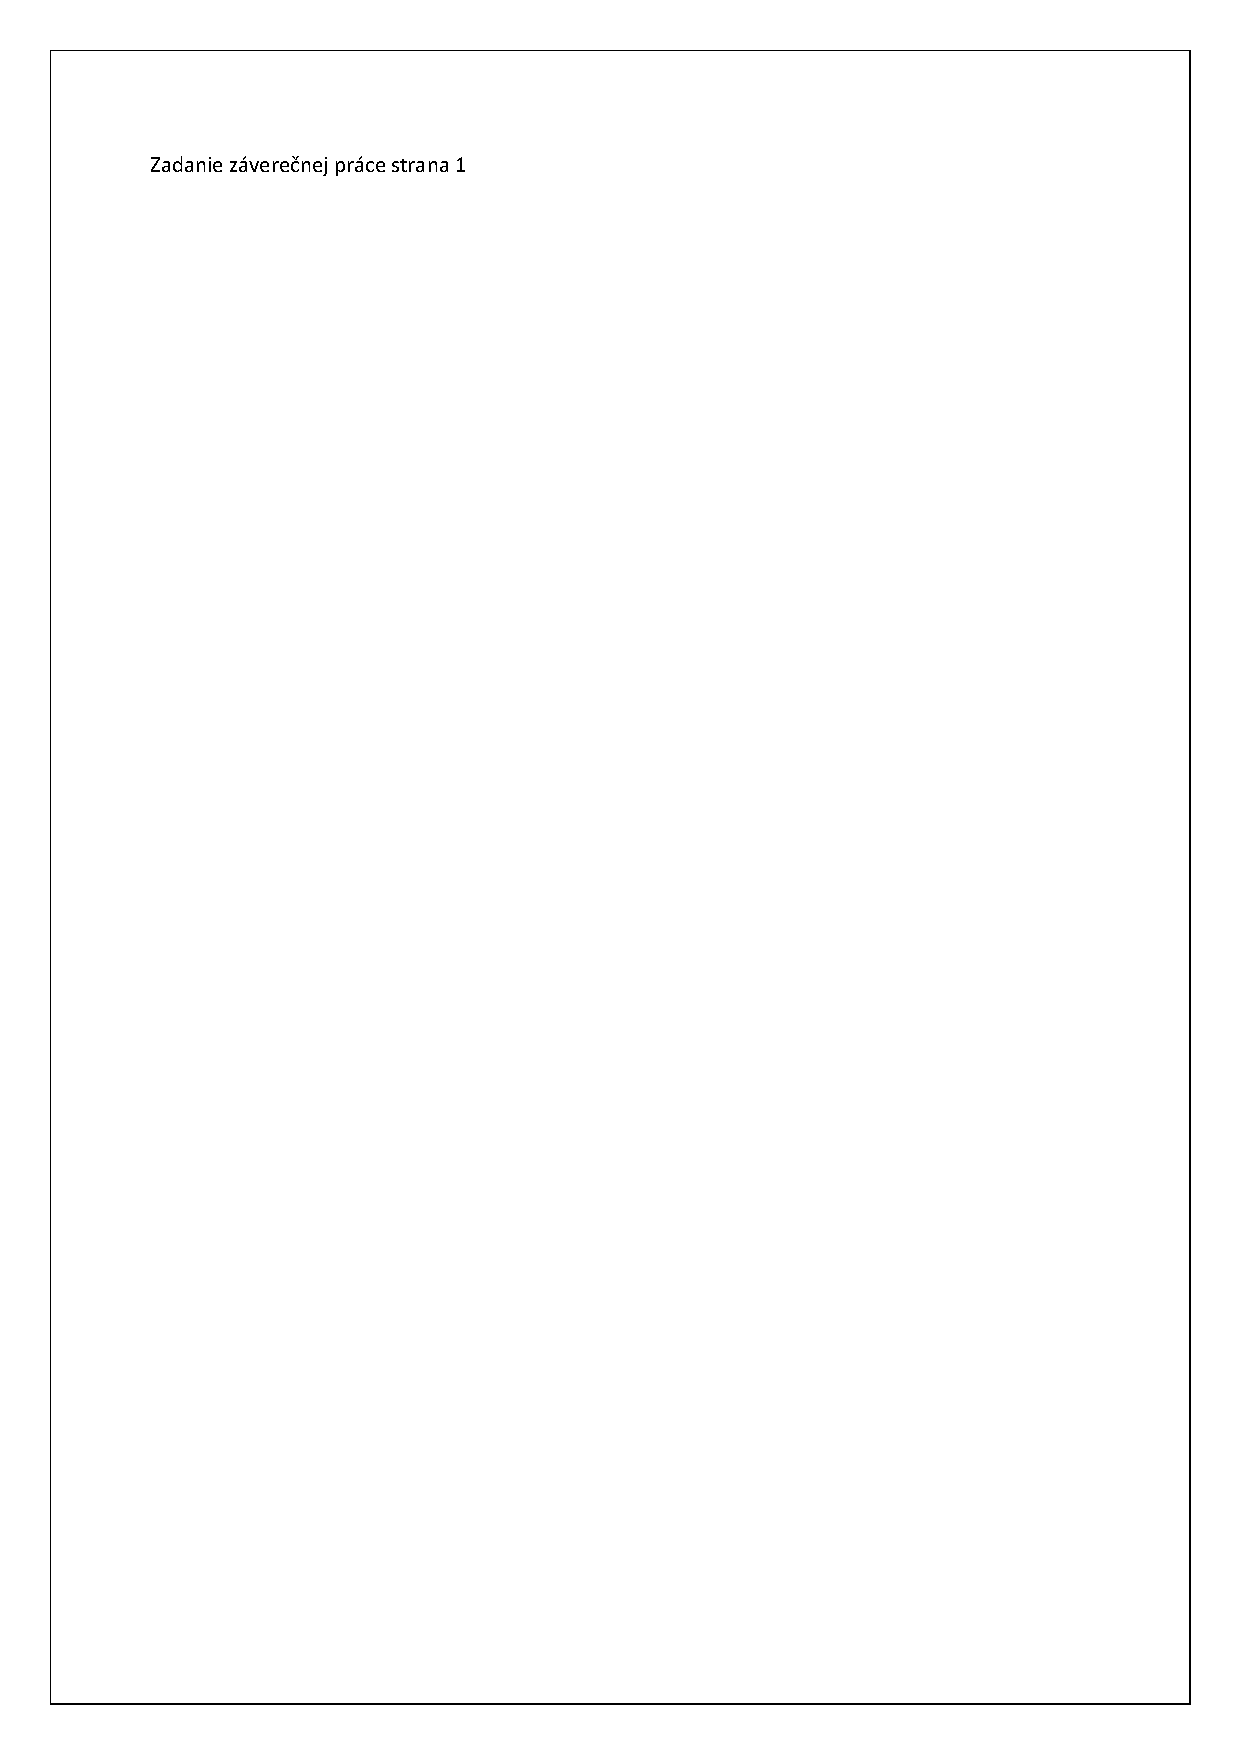
\includepdf[page=1]{content/assignment.pdf}
% use this command only if your assignment has more than 2 pages
% 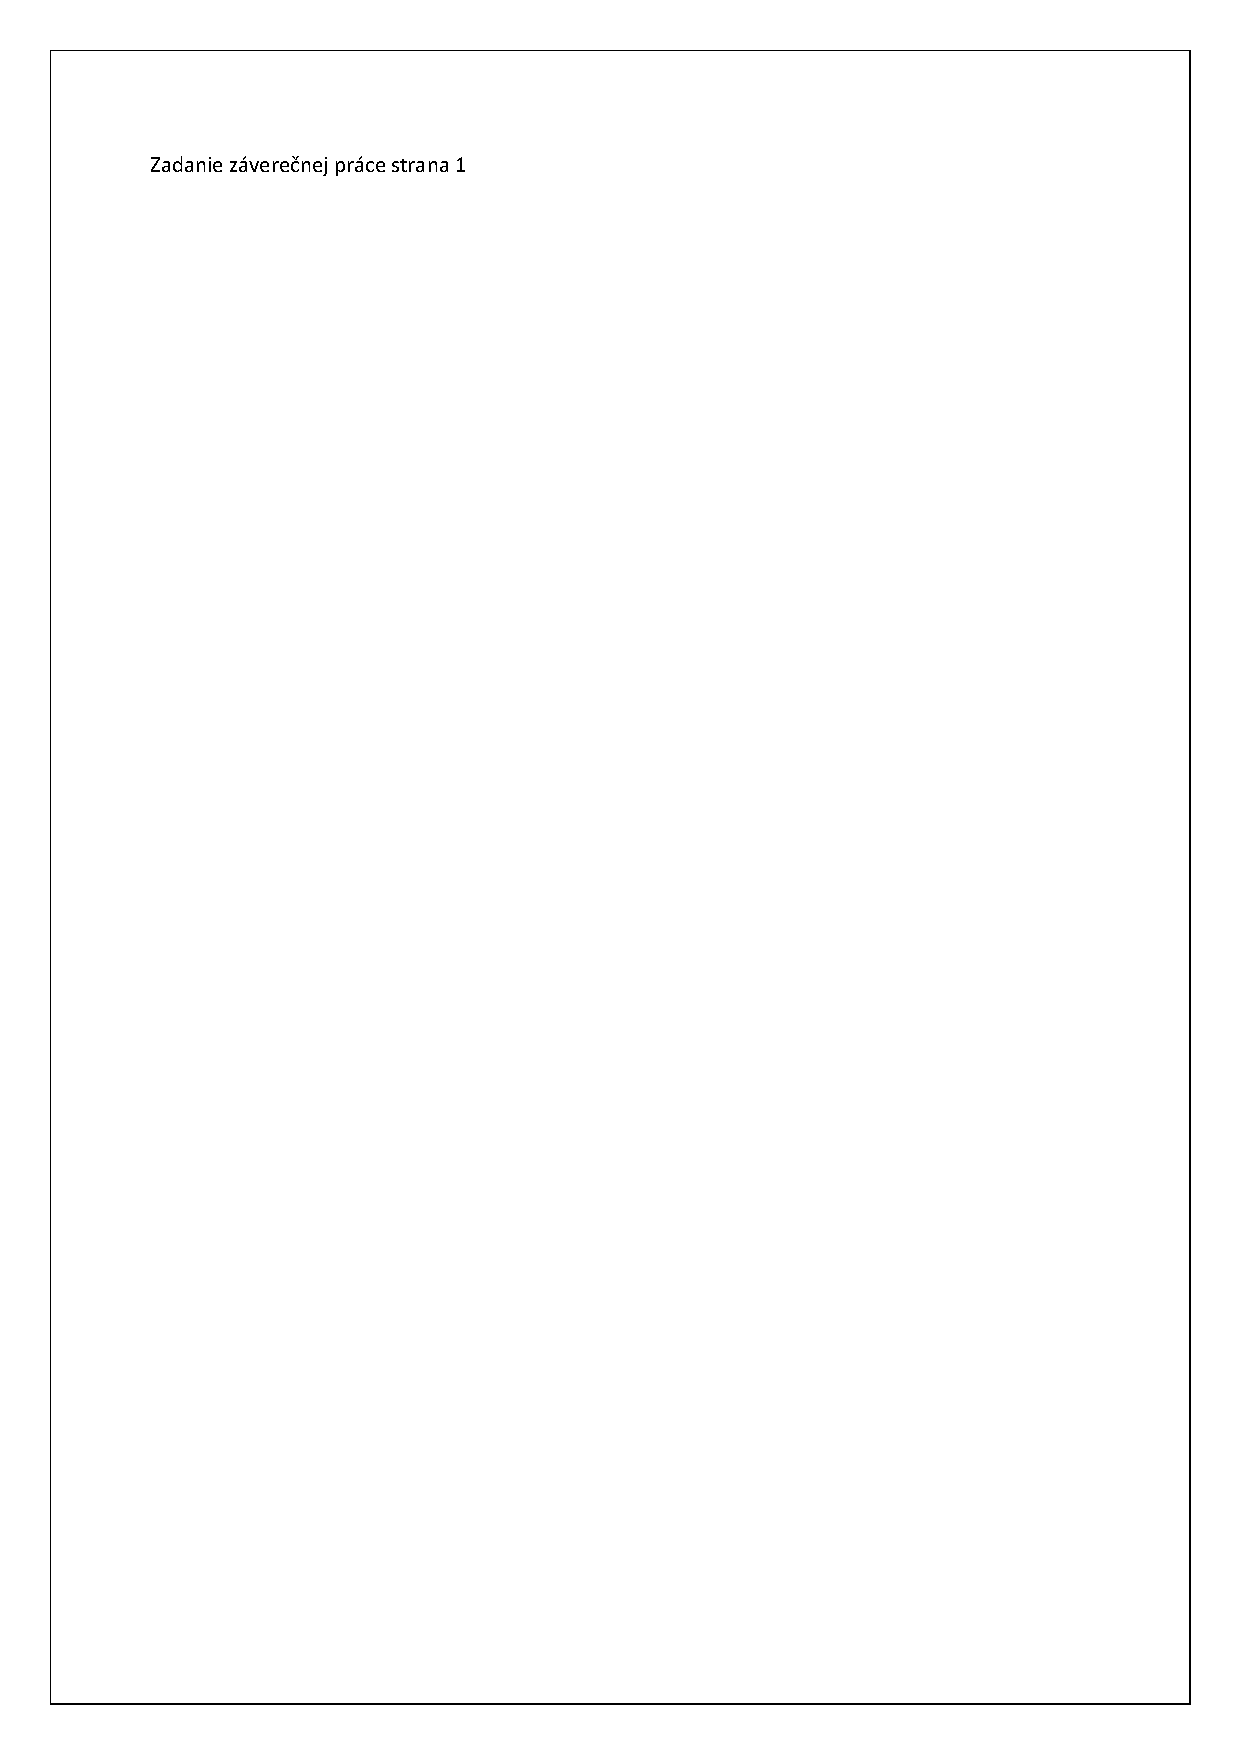
\includepdf[page=2]{content/assignment.pdf}


% do not remove following commands
% do not following commands
\chapter*{\thesisack}
\markboth{}{}
\addcontentsline{toc}{chapter}{\thesisack}
Write here the acknowledgment

\chapter*{Abstract}
\markboth{}{}
\addcontentsline{toc}{chapter}{Abstract}
The different behavior of the real plant and its mathematical description is a relatively well-known issue in the field of automation, which is a serious problem, especially in a situation where we try to ensure optimal operation of the plant. Many scientific publications address this issue, but the solutions they offer are often very complicated to implement or lead to uncertain results. This work brings a new approach to the model--plant mismatch optimization, which is based on hybrid modeling using the method of guaranteed parameter estimation. We decided to demonstrate the functionality of this method on a plant that is represented by a chemostat, because it offers many problems with modeling due to the presence of living organisms. The basic idea is to supplement the discrepancies between the real plant (Monod model) and the inaccurate mechanical model (Haldane model) using data models, which were identified on the data described by these differences.

The results of the experiments showed that hybrid models can be used to optimize the operation of the plant, but  with an iterative approach they are not able to ensure convergence to the real optimal steady state of the plant, only to its immediate surroundings. Unlike the modifier adaptation scheme, the convergence of hybrid models is significantly faster and less sensitive to measurement noise, which is a great advantage for processes with large time constants.

\chapter*{Abstrakt}
\markboth{}{}
\addcontentsline{toc}{chapter}{Abstrakt}
Slovenský abstrakt

\setcounter{tocdepth}{2}
\renewcommand{\baselinestretch}{0.1}\normalsize
\tableofcontents
\renewcommand{\baselinestretch}{1.1}\normalsize



% ----------------------------------------------------------------%
% The Mainmatter !! Do NOT change the structure!!                 %
% ----------------------------------------------------------------%
\mainmatter

% individual chapters should be included via a separate tex file, as shown in 
% here. When working in TexStudio (recomennded tool for Win and Mac) set the 
% main.tex as an Explicit root document, so you can compile even you are
% working on other chapter in other tex file.
%
% Open main.tex THEN click Options-> Root Document -> Set Current Document as
% Explicit Root

% introduction
\chapter*{Úvod}
\addcontentsline{toc}{chapter}{Úvod}
V tomto momente, ako čítate tento text, prebieha okolo nás množstvo procesov, ktoré zabezpečujú fungovanie dnešnej spoločnosti bez toho, aby si to človek vôbec uvedomoval a ťažko povedať, či si ešte dokážeme predstaviť život bez týchto vymožeností. O čom je reč ? Distribúcia elektrickej energie, pitnej vody, plynu, separácia odpadu či čistenie odpadových vôd alebo každodenný prísun potravín, liečiv, pohonných hmôt, oblečenia atď. Asi je zrejmé, že takto by sme mohli pokračovať ešte veľmi dlho. Čo sa však snažíme ozrejmiť je, že väčšina týchto procesov je nejakým spôsobom automatizovaná, čo nám umožňuje vykonávať daný proces efektívne, kvalitne a hlavne bezpečne. 

Základným kameňom väčšiny pokročilejších metód automatizácie je matematický model zariadenia. V princípe existujú dva prístupy k matematickému modelovaniu. Prvý prístup je založený na fyzikálnych zákonoch, ktorý vedie k tak zvaným mechanickým modelom. Problémom takéhoto modelovania je, že s rastúcimi požiadavkami na kvantitu, kvalitu, bezpečnosť alebo efektivitu, rastie aj zložitosť priemyselných procesov -- jednak štruktúra zariadenia a jednak stupeň automatizácie, čo vedie ku komplikáciám. Nehovoriac o tom, že takýto prístup je časovo a aj finančne veľmi náročný. Druhý prístup vychádza z analýzy a identifikácie veľkého množstva nameraných procesných údajov, čo vedie k dátovým modelom. Dátové modely sú jednoduchšie na konštrukciu, avšak môžu so sebou prinášať neistoty v podobe nesprávnej štruktúry modelu alebo parametrov. Tieto neistoty sú najčastejšie spôsobené vplyvom chyby merania.

Existuje viacero metód, ktoré dokážu spracovať zašumený signál, a každá z nich so sebou nesie určité nevýhody. Napríklad metóda najmenších štvorcov predpokladá, že šum merania má normálne rozdelenie a ak tento predpoklad nie je dodržaný, môže viesť k nesprávnym výsledkom.

Garantovaný odhad parametrov (GOP) je metóda, ktorá obchádza problém poznania rozdelenia náhodných veličín a namiesto toho predpokladá ľubovoľnú ale ohraničenú chyba merania. Výsledkom identifikácie pomocou GOP sú intervalové odhady parametrov modelu, ktoré zabezpečia, že nameraný výstup procesu sa bude nachádzať v rozmedzí stanovenej chyby merania.  

Tu sa naskytá otázka, či by nebolo možné opísať komplikované zariadenie jednoduchším mechanickým modelom a vzniknuté rozdiely od skutočného zariadenia doplniť dátovými modelmi. Ako bolo ukázané vo viacerých vedeckých publikáciach, takéto hybridné modely je možné skonštruovať a využiť ich v rôznych oblastiach automatizácie \cite{hamilton:hybrid_modeling:2017}, \cite{hernandez:economics_opt_w_mismatch:2019}. Výhodou hybridných modelov je väčšia robustnosť a krátkodobá predikcia, najmä v situáciách, kde je veľká neistota v parametroch modelu \cite{hamilton:hybrid_modeling:2017}.

Hlavným predmetom tejto práce je ukázať ako možno skonštruovať hybridný model využitím metódy garantovaného odhadu parametrov a aplikovať ho pri ekonomickej optimalizácii dynamického procesu prietokového biochemického reaktora.

Biochemické reaktory sa považujú za dôležitú súčasť chemického priemyslu. Široká škála dôležitých zlúčenín ako farmaceutické produkty, rôzne polyméry alebo produkty potravinárskeho priemyslu sa vyrábajú pomocou určitého fermentačného média (rôzne baktérie, kvasinky, vláknité huby alebo enzýmy) za prísne stanovených podmienok v biochemickom reaktore \cite{srinivasan:chemostat_opt:2003}. Na druhej strane, biochemické reaktory vykazujú širokú škálu dynamického správania a ponúkajú veľa problémov s modelovaním v dôsledku prítomnosti živých organizmov, ktorých rýchlosť rastu je opísaná komplexnými kinetickými výrazmi \cite{psichogios:hybrid_process_model:1992}.


% theory

	% PART 1 - GPE
	%datove modelovanie
	\part{Dátové modelovanie a Garantovaný odhad parametrov}
\chapter{Dátové modelovanie}
V dnešnom svete sme doslova obklopený množstvom dát, ktoré vychádzajú z rôznych zariadení. Tieto dáta sa dajú použiť rôzne --- štúdium procesov (Čo sa stalo v danom okamihu?), predikcia udalostí (Čo sa môže stať?), a aj reakcia na ne (Čo môžeme spraviť?). Týmito otázkami sa zaoberá dátové modelovanie. Vo všeobecnosti by sa dalo povedať, že úlohou dátového modelovania je nájsť vzorec medzi závislou (vstupnou) a nezávislou (výstupnou) premennou, ktorý je skrytý v súbore dát --- extrahuje model z údajov bez akýchkoľvek predpokladov na funkčnosť, čím sa môže stratiť určitá miera interpretovateľnosti modelu, ale vo všeobecnosti sa uľahčí prístup k matematickému modelovaniu~\cite{mishra:data_modeling:2018}.

Raz uviedol známy matematik a štatistik George E.P. Box  v jednej z jeho publikácii nasledovný citát: \aps{\textit{Všetky modely sú nesprávne, ale niektoré sú užitočné.}}~\cite{box:sas:1976}. Nejde iba o slaboduchú dehonestáciu dátového modelovania. Týmto citátom chcel vyjadriť skutočnosť, že samotné modely, už z definície, sú iba aproximáciami neznámej reality --- neexistuje žiaden pravý model, ktorý by dokázal perfektne reflektovať skutočnosť. Okrem toho kvalita modelu závisí od veľkosti vzorky dát -- menšie efekty je možné odhaliť iba pri zväčšovaní veľkosti vzorky. Množstvo informácií vo veľkých súboroch údajov výrazne prevyšuje informácie v malých vzorkách dát~\cite{kenneth:understanding_stand_crit:2004}. Toto je daň, ktorú platíme za \aps{jednoduchosť} dátového modelovania.

\section{Dátové modely}
V tejto časti si uvedieme niektoré základné formulácie modelov lineárnych dynamických systémov v diskrétnom čase, ktoré sa najčastejšie používajú pri identifikácii nameraných údajov. Najskôr je však nutné zaviesť pojem ARMA proces, na základe ktorého môžeme vyjadriť ľubovoľný stacionárny náhodný signál ako biely šum prechádzajúci lineárnym systémom~\cite{fikar:identifikacia:1999}.

\textbf{ARMA proces} 
\newline
Uvažujme proces $y(t)$, ktorý môže byť reprezentovaný ako biely šum $ e(t) $ prechádzajúci lineárnym systémom v tvare 
\begin{equation}
	y(t) = F(q)e(t),
\end{equation}
kde $q$ je operátor posunutia a $F(q)$ je racionálna lomená funkcia v tvare 
\begin{equation}
	F(q) = \frac{C(q)}{A(q)} = \frac{1 + \sum_{i=1}^{n_c} c_{i}q^{-i}}{1 + \sum_{i=1}^{n_a} a_{i}q^{-i}},
\end{equation}
kde $n_c$ resp. $n_a$ predstavuje rád čitateľa resp. rád menovateľa. Pri takejto formulácii, ARMA proces vyzerá nasledovne 
\begin{equation}
	\begin{split}
			y(t) = &-a_{1}y(t-1) - \dots -a_{n_a}y(t-n_a) + \\
				   &+e(t) + c_1e(t-1) + \dots + c_{n_c}e(t-n_c).
	\end{split} 
\end{equation}
Skladá sa z dvoch častí --- AR (autoregressive), keď $n_c = 0$
\begin{equation}
	y(t) + a_{1}y(t-1) + \dots + a_{n_a}y(t-n_a) = e(t)
\end{equation}
a z časti MA (moving average), keď $n_a = 0$
\begin{equation}
	y(t) = e(t) + c_1e(t-1) + \dots + c_{n_c}e(t-n_c).
\end{equation}
Zatiaľ čo AR opisuje dynamiku výstupu $ y(t) $, zložka MA modeluje vplyv poruchovej veličiny $ e(t) $.
 
\textbf{ARX model}
\newline
 ARX (Autoregressive with eXogenous variable) model predpokladá, že skutočný dynamický systém je popísaný diferenčnou rovnicou v tvare
 \begin{equation}
 	y(t) = \frac{B(q)}{A(q)}u(t) = \frac{\sum_{i=1}^{n_b} b_{i}q^{-i}}{1 + \sum_{i=1}^{n_a} a_{i}q^{-i}}u(t),
 \end{equation}
 čo môžeme prepísať do tvaru 
 \begin{equation}
	 \begin{split}
		 y(t) = &- a_{1}y(t-1) - \dots - a_{n_a}y(t-n_a) + \\
		 		&+ b_{1}u(t-1) + \dots + b_{n_b}u(t-n_b) + e(t), 
	 \end{split}
	 \label{eq:ARX_m} 
 \end{equation}
 kde $ y(t) $ sú výstupy modelu a $ u(t) $ sú jeho vstupy. ARX model predpokladá, že chyba vstupuje do rovnice systému v podobe bieleho šumu $ e(t) $.
 
 \textbf{FIR model}
 \newline
 FIR (Finite Impulse Response) je špeciálny prípad ARX modelu práve tedy, ak rád menovateľa $n_a = 0$. Takýto model je závislý iba od vstupov a môžeme ho opísať diferenčnou rovnicou v tvare
 \begin{equation}
 	\begin{split}
 		y(t) &= B(q)u(t) = \sum_{i=1}^{n_b} b_{i}q^{-i}u(t) = \\
 			 &= b_{1}u(t-1) + \dots + b_{n_b}u(t-n_b).
 	\end{split}
 	\label{eq:FIR_m}
 \end{equation}
 
 \textbf{ARMAX model}
 \newline
 Ide o modifikovaný ARX model, kde sa predpokladá, že chyba vstupuje ako MA model. Výsledný tvar je nasledovný 
 \begin{equation}
	 \begin{split}
		 y(t) = &- a_{1}y(t-1) - \dots - a_{n_a}y(t-n_a) + \\
		 		&+ b_{1}u(t-1) + \dots + b_{n_b}u(t-n_b) + \\
		 		&+ e(t) + c_{1}e(t-1) + \dots + c_{n_c}e(t-n_c).
	 \end{split} 
 \end{equation}
 
 \textbf{OE model}
 \newline
 Ďalším modelom v tejto sérii je OE model, teda \aps{Output Error} resp. \aps{Chyba na Výstupe}. Jeho štruktúra je podobná s ARX model, avšak s tým rozdielom, že OE model obsahuje vnútornú premennú $w(t)$, ktorá nie je priamo pozorovateľná a preto sa musí odhadovať
 \begin{equation}
	 \begin{split}
		 w(t) = &- g_{1}w(t-1) - \dots - g_{n_g}w(t-n_g) + \\
		 		&+ b_{1}u(t-1) + \dots + b_{n_b}u(t-n_b), \\
		 y(t) = &\quad w(t) + e(t).
	 \end{split} 
 \end{equation}
 
 \textbf{Box-Jenkinsov model}
 \newline
 Všeobecnejšia forma OE modelu predstavuje Box-Jenkinsov model, kde šum na výstupe je modelovaný ako ARMA proces
 \begin{equation}
 	y(t) = \frac{B(q)}{G(q)}u(t) + \frac{C(q)}{D(q)}e(t).
 \end{equation}
 
\textbf{Všeobecný model}
\newline 
Predstavuje najviac zovšeobecnenú formu, ktorá je vyhovujúca pre všetky uvedené modely
\begin{equation}
	A(q)y(t) = \frac{B(q)}{G(q)}u(t) + \frac{C(q)}{D(q)}e(t).
\end{equation}

	\section{Odhad parametrov}
Podobne dôležitá ako samotná štruktúra resp. voľba dátového modelu, je aj odhad jeho parametrov. V tejto časti spomenieme niektoré z najviac využívaných metód na identifikáciu či už statických alebo dynamických modelov. 

Skôr ako začneme rozoberať samotné metódy, je potrebné spomenúť základné požiadavky na odhad parametrov~\cite{beck:param_est:1977}, ktoré by mala každá dobrá metóda spĺňať. Tieto požiadavky tvoria súhrn štatistických vlastností, ktoré chceme, aby daná metóda mala, pretože vedú k správnemu, možno by bolo lepšie povedať k optimálnemu, odhadu parametrov.

\subsection{Požiadavky na odhad parametrov}
Majme vektor $ \hat{\theta} $, ktorý predstavuje vektor odhadnutých parametrov $ \theta $, potom:
\begin{itemize}
	\item[] \textbf{nevychýlenosť} odhadu definujeme ako
	\begin{equation*}
		E\left\lbrace \hat{\theta}^k \right\rbrace = \theta, 
	\end{equation*}
	čo znamená, že ak odhad parametrov uskutočníme na základe $ k $ meraní, potom pre každé meranie $ k $ musí platiť, že stredná hodnota odhadnutých parametrov $ E\left\lbrace \hat{\theta}^k \right\rbrace $ sa rovná ich skutočným hodnotám $ \theta $.
	\item[] \textbf{konzistencia} znamená, že pre ľubovoľný vektor konštánt $ \delta > 0 $ platí
	\begin{equation*}
		\lim\limits_{k \rightarrow \infty} P \left( \left| \hat{\theta}^k - \theta \right| < \delta \right) = 1. 
	\end{equation*}
	Táto definícia v podstate tvrdí, že so zväčšujúcim sa počtom dát, by sa odhad parametrov mal zlepšovať resp. by sa mal blížiť ku skutočným hodnotám (pravdepodobnosť, že absolútna hodnota rozdielu odhadovaných a skutočných parametrov $ P \left( \left| \hat{\theta}^k - \theta \right| \right) $ bude ležať v ľubovoľnom $ \delta $ okolí, bude mať hodnotu istého javu).
	\item[] \textbf{výdatnosť}, t.j., ak medzi odhadom $ \hat{\theta} $ a ľubovoľným ďalším odhadom $ \tilde{\theta} $ platí 
	\begin{equation*}
		\text{Cov} \left( \tilde{\theta} \right) - \text{Cov} \left( \hat{\theta} \right) \geq 0,
	\end{equation*}
	teda optimálny odhad je ten, ktorý má minimálnu disperziu resp. kovarianciu $ \text{Cov} \left(\right) $ (v skalárnom prípade). Pri nulovej disperzii prechádza pravdepodobnosť v istotu. Výdatnosť sa v literatúre môže označovať taktiež ako efektívnosť \cite{beck:param_est:1977}.
\end{itemize}

\subsection{Metódy statickej identifikácie}
\subsubsection*{Metóda najmenších štvorcov}
Jednou z najpoužívanejších metód, ktorú vynašiel Gauss pri výpočte obežných dráh komét a planét z nameraných údajov, je metóda najmenších štvorcov \cite{hostetter:recursive_est:1987}. Princíp tejto metódy je založený na hľadaní takej kombinácie parametrov systému, ktorá minimalizuje vzdialenosť medzi nameranými a odhadnutými údajmi. Treba zdôrazniť, že táto metóda vyžaduje, aby parametre modelu boli v lineárnom vzťahu k vstupom.

Začnime nasledovne. Majme systém $ F(\theta, x) $, ktorý je funkciou vstupov modelu $ x $ a parametrov $ \theta $. Výstup $ y $ z takéhoto systému, ktorý je zaťažený chybou merania $ e $, je
\begin{equation}
	y = \theta^T x + e = \theta_1x_1 + \theta_2x_2 + \dots + \theta_kx_k.
\end{equation}
Pokúsme sa nájsť, takú hodnotu parametrov $ \hat{\theta} $, ktorá by minimalizovala súčet druhých mocnín odchýliek nameraných údajov od modelových výstupov ako
\begin{equation}
	J\left(\theta\right) = \sum_{i=1}^{k} e_i^2 = \sum_{i=1}^{k} \left(y_i - \theta^T x_i\right)^2.
\end{equation}
Túto rovnicu môžeme napísať vo vektorovom tvare
\begin{equation}
	J\left(\theta\right) = \left(Y - X\theta \right)^T \left(Y - X\theta \right).
\end{equation} 
Formálne sa rovnica nezmenila, iba sme zadefinovali dva nové vektory
\begin{equation}
	Y = \begin{pmatrix}
			y_1 \\
			y_2 \\
			\vdots \\
			y_k
		\end{pmatrix}, \qquad
	X = \begin{pmatrix}
			x_1^T \\
			x_2^T \\
			\vdots \\
			x_k^T
		\end{pmatrix}.
\end{equation}
Podmienku minima zabezpečíme z nulovej hodnoty gradientu funkcie $ J(\theta) $ podľa $ \theta $.
\begin{equation}
	\nabla J \left(\theta\right) = \frac{\partial J \left(\theta\right)}{\partial \theta} = -X^T Y + X^T X\hat{\theta} = 0.
\end{equation}
Z toho jasne vyplýva, že ak existuje inverzia výrazu $ X^T X $, vektor odhadovaných parametrov získame ako 
\begin{equation}
	\hat{\theta} = \left(X^T X\right)^{-1}X^T Y.
\end{equation}
Bez dôkazu uvádzame, že metóda najmenších štvorcov spĺňa všetky požiadavky na odhad parametrov \cite{fikar:identifikacia:1999}.

\subsubsection*{Modifikovaná metóda najmenších štvorcov}
V prípade, že náhodný šum $ e $ je korelovaný a poznáme jeho kovariančnú maticu $ \Sigma $, môžeme prepísať kritérium minimalizácie do tvaru 
\begin{equation}
	J\left(\theta\right) = \left(Y - X\theta \right)^T \Sigma^{-1} \left(Y - X\theta \right).
\end{equation}
Ak uvažujeme stochastický proces, potom najlepší nevychýlený odhad parametrov $ \hat{\theta} $ získame ako
\begin{equation}
	\hat{\theta} = \left(X^T \Sigma^{-1} X\right)^{-1}X^T \Sigma^{-1} Y.
\end{equation}
Takúto modifikáciu metódy najmenších štvorcov používame najmä vtedy, ak sa v meraní vyskytujú systematické chyby, zaznamenávanie nameraných údajov má časové oneskorenie, disponujeme nesprávnym modelom, zvolili sme nesprávne vstupné veličiny alebo namerané dáta boli nejakým spôsobom filtrované alebo extrapolované \cite{fikar:identifikacia:1999}.

\subsubsection*{Formulácia vhodnej optimalizačnej úlohy}
Metóda najmenších štvorcov, napriek tomu ako veľmi elegantne si dokáže poradiť s odhadom parametrov, má jednú veľkú nevýhodu. Parametre modelu musia byť v lineárnom vzťahu ku vstupom, pričom samotné vstupy môžu predstavovať ľubovoľné lineárne aj nelineárne funkcie. Týmto sa eliminuje značná časť problematík, ktoré jednoducho nedokáže vyriešiť. 

Ukazuje sa, že vhodným definovaním optimalizačného problému, dokážeme spomenutý problém obísť a nie len to. Takýto prístup nám umožňuje odhadovať parametre dynamických systémov, teda diferenciálnych alebo diferenčných rovníc \cite{villaverde:opt_param_est:2018}.

Majme ľubovoľnú diferenciálnu rovnicu
\begin{equation}
	\dot{x}(t) = f\left( t, x(t), \theta \right),
\end{equation} 
a súbor nameraných údajov $ y = [y_1, y_2, \dots , y_N] $ z daného dynamického systému. Budeme hľadať takú kombináciu parametrov $ \hat{\theta} $, ktorá minimalizuje sumu kvadrátu rozdielu nameraných a modelových údajov. Odhad parametrov potom získame ako
\begin{equation}
	\begin{split}
		\hat{\theta} = \arg \min_{\theta} \quad & \sum_{i=1}^{N} \left(y_{i} - x(t_{i})\right)^2. \\
		\textrm{s.t.} \quad & \dot{x}(t) = f\left(t,x(t),\theta \right)\\
		 & x(0) = x_0
	\end{split}
	\label{eq:param_est_opt_form}
\end{equation} 
Ako si môžeme všimnúť, účelová funkcia takto zadefinovanej optimalizačnej úlohy a metódy najmenších štvorcov je totožná. Rozdiel je v tom, že zatiaľ čo pri metóde najmenších štvorcov sme boli schopný nájsť analytické riešenie, v tomto prípade je nutné riešiť danú optimalizačnú úlohu numericky a takýto prístup k odhadu parametrov je výpočtovo náročnejší.


	\chapter{Garantovaný odhad parametrov}
V predošlej časti sme spomenuli niekoľko metód na odhad parametrov a každá si so sebou nesie určité nároky na namerané údaje. Napríklad taká metóda najmenších štvorcov predpokladá, že šum merania má normálne rozdelenie. Čo sa stane, ak tento predpoklad alebo ďalšie, ktoré sme uviedli v časti \aps{Požadavky na odhad parametrov}, nebude dodržaný ? Je zrejmé, že to povedie k nesprávnym výsledkom. 

Zostáva tu však ešte jeden problém, ktorý je omnoho zložitejší ako samotný odhad parametrov, a tým je voľba štruktúry dátového modelu. Pomocou metódy najmenších štvorcov môžeme odhadovať parametre modelu ľubovoľnej štruktúry, v prípade že je zabezpečená linearita. Ale ako zistíme, či daný model nezanedbáva dôležitú časť dynamiky procesu alebo na druhej strane, či už neaproximuje šum merania ? Riešenie môže ponúknuť práve metóda garantovaného odhadu parametrov.

Garantovaný odhad parametrov (GOP) je metóda, ktorá obchádza problém poznania rozdelenia náhodných veličín a namiesto toho predpokladá ľubovoľnú ale ohraničenú chybu merania. Výsledkom identifikácie pomocou GOP sú intervalové odhady parametrov modelu, ktoré zabezpečia, že nameraný výstup procesu sa bude nachádzať v rozmedzí stanovenej chyby merania \cite{paulen:gpe:2017}. Demonštrujme si fungovanie tejto metódy na nasledujúcom príklade.

\section{Grafická metóda GOP}
Predstavme si, že sme získali vstupné $ u $ a výstupné $ y $ údaje z procesu, ktoré v tomto prípade budú predstavovať konštantnú funkciu, tak ako to je zobrazené na Obr. \ref{gpe_ex1_data}. Vieme, že senzor má stanovenú chybu merania $ e $. Štruktúru modelu procesu, z ktorého sme získali údaje, nepoznáme a preto sa rozhodneme, že budeme tieto údaje aproximovať lineárnym modelom
\begin{equation}
	\hat{y}(u) = \theta_1 + \theta_2u.
\end{equation}
 Jediné neznáme v tomto modely sú parametre $ \theta_1 $ a $ \theta_2 $. Na ich identifikáciu využijeme grafickú metódu GOP a začneme tým, že si vyjadríme parameter $ \theta_2 $ ako funkciu nameraných údajov $ y, u $ a parametra $ \theta_1 $
\begin{equation} \label{gpe:ex_lin_model}
	\theta_2 = \frac{1}{u}y - \frac{1}{u}\theta_1,
\end{equation}
kde $ \theta_2 $ teraz predstavuje nezávislú premennú a $ \theta_1 $ závislú. Cieľom odhadu parametrov bude, aby ich vzájomná kombinácia viedla k výstupným údajom modelu $ \hat{y}(u) $, ktoré budú ležať v rozmedzí hraníc chyby merania senzora. Táto podmienka upravuje rovnicu \ref{gpe:ex_lin_model} do tvaru
\begin{equation} 
	\theta_2 = \frac{1}{u}\left(y \pm e\right) - \frac{1}{u}\theta_1,
\end{equation}
ktorú môžeme formálne rozpísať na dve rovnice 
\begin{equation}
	\begin{split}
		\theta_2^{(1)} =& \frac{1}{u}\left(y + e\right) - \frac{1}{u}\theta_1,\\
		\theta_2^{(2)} =& \frac{1}{u}\left(y - e\right) - \frac{1}{u}\theta_1.
	\end{split} 
\end{equation}
Tieto priamky vytyčujú oblasť vhodných kombinácií parametrov modelu $ \theta_1, \theta_2 $ ktorými môžeme opísať dané dáta a garantuje, že správne riešenie leží niekde vo vnútri tejto oblasti.

\begin{figure}
	\centering
	\begin{subfigure}[b]{0.48\textwidth}
		\centering
		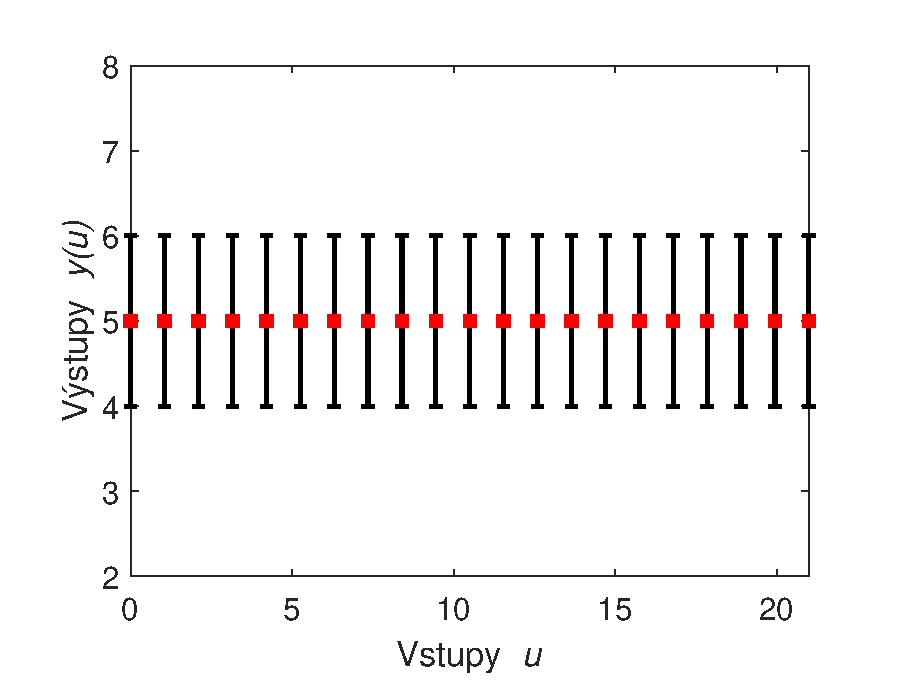
\includegraphics[width=\linewidth]{images/gpe_ex_data1}
		\caption{Namerané výstupné údaje z neznámeho procesu.}
		\label{gpe_ex1_data}
	\end{subfigure}
	\begin{subfigure}[b]{0.48\textwidth}
		\centering
		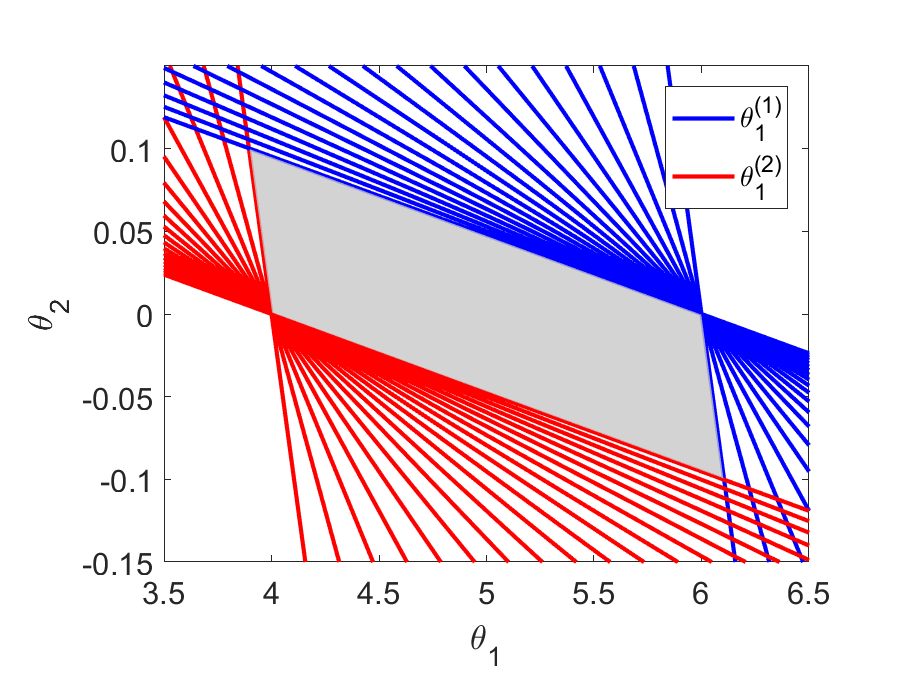
\includegraphics[width=\linewidth]{images/gpe_ex_line1}
		\caption{Grafická metóda garantovaného odhadu parametrov.}
		\label{gpe_ex1_gm}
	\end{subfigure}
	\caption{Ilustračný príklad garantovaného odhadu parametrov -- variant 1 -- zidealizovaný prípad.}
	\label{gpe_ex1}
\end{figure}

Takto sme získali nielen informácie o parametroch nášho modelu, ale aj informácie o zložitosti resp. jednoduchosti štruktúry modelu. Na Obr. \ref{gpe_ex1_gm} vidíme, že parameter $ \theta_2 $ obsahuje vo svojom intervale nulu, čím sa porušuje invariantnosť štruktúry modelu a môžeme tvrdiť, že takýto matematický opis je potenciálne zbytočne zložitý. Rovnaké dáta by sme teda vedeli opísať aj konštantným modelom, t.j. 
\begin{equation}
	\hat{y}(u) = \theta_1.
\end{equation}

 Avšak dáta zobrazené na Obr. \ref{gpe_ex1} boli trošku zidealizované a pravdepodobne v bežnom živote by nenastala situácia, že by senzor niekoľkokrát po sebe nameral tú istú hodnotu. Pozrime sa však, čo sa stane, ak naše namerané údaje budú mať bližšie k realite, tak ako je uvedené na Obr. \ref{gpe_ex2_data}. Ako si môžeme všimnúť na Obr. \ref{gpe_ex2_gm}, odhadované ohraničenie jednotlivých parametrov $ \theta_1, \theta_2 $ sa nám výrazne zmenšilo. Takže môžeme tvrdiť, že samotný šum merania nám prispieva k presnosti odhadu parametrov. 

\begin{figure}
	\centering
	\begin{subfigure}[b]{0.48\textwidth}
		\centering
		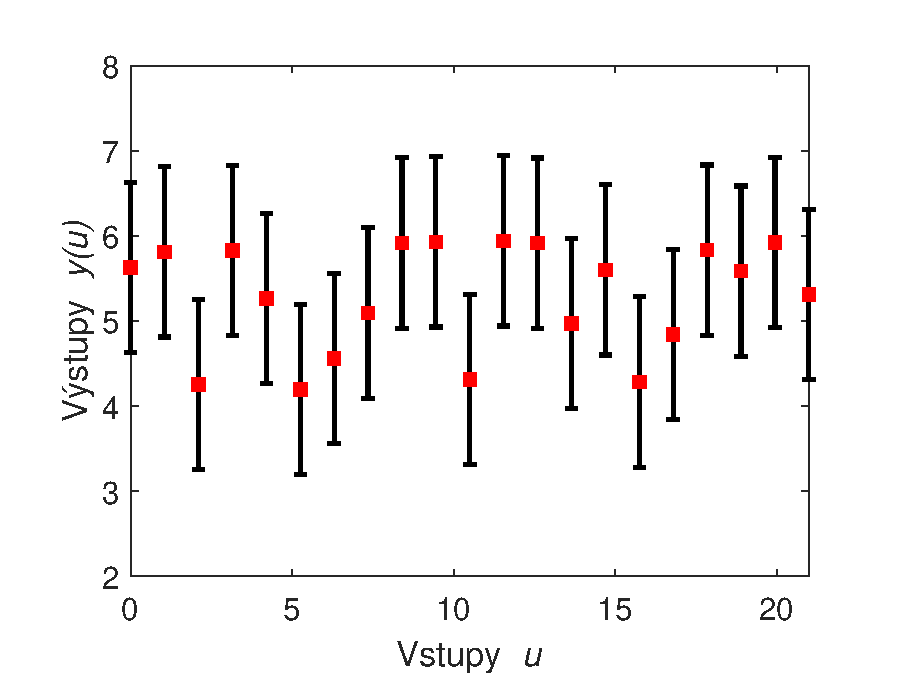
\includegraphics[width=\linewidth]{images/gpe_ex_data2}
		\caption{Namerané výstupné údaje z neznámeho procesu.}
		\label{gpe_ex2_data}
	\end{subfigure}
	\begin{subfigure}[b]{0.48\textwidth}
		\centering
		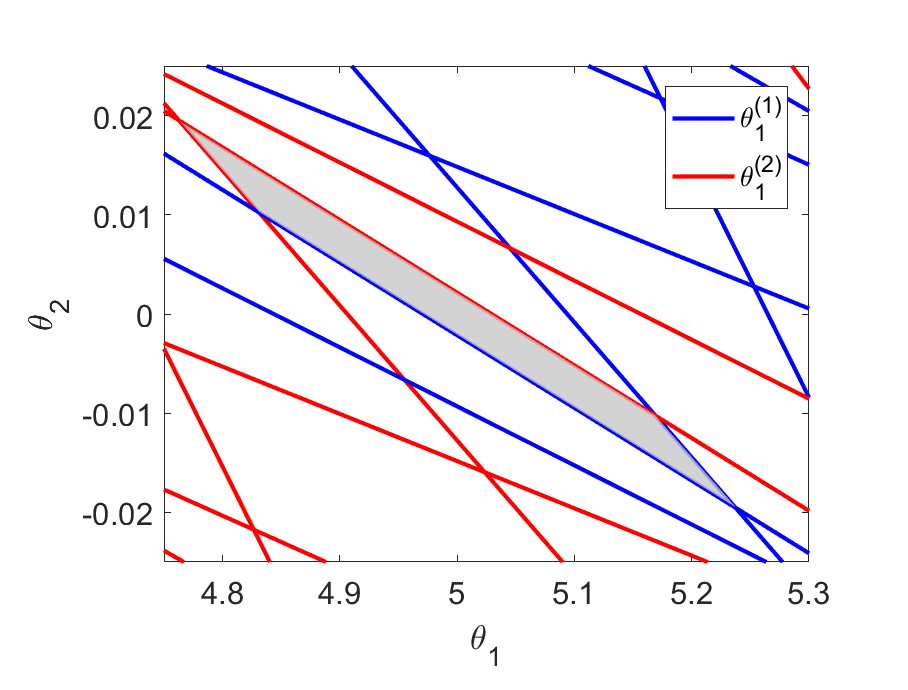
\includegraphics[width=\linewidth]{images/gpe_ex_line2}
		\caption{Grafická metóda garantovaného odhadu parametrov.}
		\label{gpe_ex2_gm}
	\end{subfigure}
	\caption{Ilustračný príklad garantovaného odhadu parametrov -- variant 2.}
	\label{gpe_ex2}
\end{figure}

\section{Mnohorozmerový prípad}
Grafická metóda GOP je krásny ilustračný príklad toho ako táto metóda funguje. Problémom však ostáva, že ak by sme potrebovali odhadovať viac parametrov ako 3 (pri bežných regresných analýzach dátových modelov potrebujeme odhadovať desiatky, možno až stovky parametrov), narážame na obmedzenia tejto metódy -- problém s vizualizáciou. Preto je nutné túto grafickú metódu vymeniť za niečo iné, čo bude obchádzať problematiku s vizualizáciou. Schodnou cestou je transformovať úlohu GOP na optimalizačnú problematiku \cite{artzova:gpe_moving_hor:2019}, ktorý by mohla vyzerať nasledovne 
\begin{equation}
	\begin{split}
		\left[ \ubar{\theta}_i, \bar{\theta}_i \right] = \min_{\theta} / &\max_{\theta} \quad \theta_i, \quad\qquad \forall i = 1,2, \dots n_y, \\
		\text{s.t.}& \quad \ubar{e} \leq y - \hat{y} \leq \bar{e}	
	\end{split}
	\label{eq:gpe:general_form}
\end{equation} 
kde 
\begin{equation*}
	\theta = 
	\begin{pmatrix}
		\ubar{\theta}_1 & \bar{\theta}_1 \\
		\ubar{\theta}_2 & \bar{\theta}_2 \\
		\vdots & \vdots \\
		\ubar{\theta}_{n_y} & \bar{\theta}_{n_y}	
	\end{pmatrix}.
\end{equation*}

Takto hľadáme minimálnu $ \ubar{\theta}_i $ resp. maximálnu $ \bar{\theta}_i $ hodnotu všetkých $ n_y $ odhadovaných  parametrov, ktoré nám zaručia, že rozdiel výstupov nameraných $ y $ a modelových $ \hat{y} $ bude ležať v hraniciach chyby merania $ \langle \ubar{e}, \bar{e} \rangle $.

\section{Odhad rádu modelu}
V predchádzajúcej časti sme ukázali ako získať intervalové hodnoty parametrov pre ľubovoľný počet odhadovaných parametrov. Čo sme však zamlčali bolo, že nie každá štruktúra modelu dokáže splniť podmienku optimalizačnej úlohy \ref{eq:gpe:general_form}. Preto, skôr ako začneme riešiť úlohu odhadu parametrov, potrebujeme odhadnúť vhodnú štruktúru resp. rád modelu. V tejto časti uvedieme ako riešiť problematiku odhadu minimálneho rádu modelu. Úlohu hľadania adekvátneho maximálneho rádu modelu objasníme v časti \aps{Verifikácia dátových modelov}.

Odhad minimálneho rádu modelu môžeme opäť sformulovať ako optimalizačný problém v tvare
\begin{equation}
	\begin{split}
		n_y \leftarrow \min_{\theta} & \quad 0, \\
		\text{s.t} & \quad \ubar{e} \leq y - \hat{y} \leq \bar{e}
	\end{split}
	\label{eq:GPE_m_order_est}
\end{equation}
kde $ \theta^T = (\theta_1, \theta_2, \dots, \theta_{n_y}) $ je vektor odhadovaných parametrov a $ n_y $ predstavuje odhadovaný minimálny rád modelu. Takáto formulácia rieši problematiku prípustnosti, ktorej cieľom je nájsť najjednoduchšiu štruktúru dátového modelu, pri ľubovoľných hodnotách parametrov $ \theta $, ktorá neporušuje ohraničenia optimalizačného problému.  

\section{Verifikácia dátových modelov}
Úlohou verifikácie dátových modelov je overiť správnosť a posúdiť kvalitu daného dátového modelu spomedzi viacerých možností. Existuje množstvo metód a prístupov, ktoré sa snažia riešiť danú problematiku. My spomedzi nich spomenieme tzv. štandardné kritéria a zobrazenie Pareto front, ktoré sa buď používajú najčastejšie, alebo dokážu túto úlohu riešiť efektívnejším spôsobom.

\subsection{Štandardné kritéria}
Pre štandardné kritéria je základným elementom výberu vhodného modelu zložitosť modelu. Tieto kritéria penalizujú pravdepodobnosť na základe počtu parametrov resp. rádu modelu a veľkosti vzorky. Akaike, v roku 1974, navrhol použitie Kullback–Leibler informačnej hodnoty na výber modelov, ktorým sa ustanovil vzťah medzi informovanosťou, pravdepodobnosťou a Kullback–Leibler maximom. Až neskôr, keď sa stanovil vzťah na odhad  Kullback–Leibler informačnej hodnoty, ju začali nazývať \aps{Akaike information criterion (AIC)} alebo Akaikeho informačné kritérium  \cite{emiliano:stand_crit:2014}. 

Postupom času pribúdali ďalšie informačné kritéria, ktoré nejakým spôsobom modifikovali AIC. Medzi ne patria AIC s korekciou, ktoré sa zvykne označovať ako \aps{AICc} a taktiež Bayesovské informačné kritérium \aps{BIC}. Pri aplikácii týchto kritérií na sadu požadovaných modelov, najlepším modelom je ten, ktorý má najnižšiu hodnotu AIC, AICc alebo BIC.

\textbf{AIC}
\newline
Toto kritérium je založené na koncepte informácie a poskytuje relatívnu mieru stratených informácií, keď sa konkrétny model používa na opis skutočného javu \cite{emiliano:stand_crit:2014}. Akaikeho kritérium možno vyjadriť nasledovne
\begin{equation}
	\text{AIC} = 2k - 2\ln\left( \hat{L} \right),
\end{equation}
kde $ k $ reprezentuje počet parametrov modelu a $ \hat{L} $ je funkcia pravdepodobnosti, ktorá vyjadruje mieru správnosti regresie dát daným modelom. Jednou z takýchto funkcií je aj funkcia hustoty pravdepodobnosti normálneho rozdelenia, ktorej tvar je 
\begin{equation}
	\hat{L} = \frac{1}{\sigma \sqrt{2\pi}}e^{-\frac{1}{2}\left( \frac{x - \mu}{\sigma} \right)^2},
\end{equation}
kde $ \mu $ je stredná hodnota rozdelenia, $ \sigma $ je jeho štandardná odchýlka a rozptyl sa označuje ako $ \sigma^2 $.

\textbf{AICc}
\newline
Nevýhodou AIC je, že môže nepresne vyhodnotiť kvalitu modelu v prípade, že počet parametrov je väčší ako veľkosť vzorky \cite{emiliano:stand_crit:2014}. Vtedy je nutné upraviť dané kritérium
\begin{equation}
	\text{AICc} = \text{AIC} + \frac{2k^2 + 2k}{n - k - 1}, 
\end{equation}
kde $ n $ predstavuje veľkosť vzorky dát. AICc by sa malo používať, ak pomer $ \frac{n}{k} $ je malý, napríklad $ \frac{n}{k} < 40$ \cite{kenneth:understanding_stand_crit:2004}. V opačnom prípade, keď je tento pomer dostatočne veľký, obe informačné kritéria by mali vracať podobné výsledky.

\textbf{BIC}
\newline
Bayesove informačné kritérium slúži na hodnotenie kvality modelu, ktoré je založené na posteriornej pravdepodobnosti porovnávaných modelov. Vychádza z Bayesovej teorii a aproximácii Laplaceových integrálov, ktoré vyjadrujú skreslenie podpornej funkcie \cite{emiliano:stand_crit:2014} a definujú dané informačné kritérium ako
\begin{equation}
	\text{BIC} = \ln\left( n \right)k - 2\ln\left( \hat{L} \right).
\end{equation}

\subsection{Pareto front}
Táto metóda je pomenovaná po talianskom inžinierovi, sociológovi, ekonómovi, politickom vedcovi a filozofovi Vilfredovi Paretovi. On si ako prvý uvedomil, že veľa ekonomických riešení pomáhajú určitej skupine ľudí, zatiaľ čo inej ubližujú. Jeho prácou sa snažil nájsť také riešenie, ktoré  by na jednej strane pomáhalo a na druhej neubližovalo \cite{mornati:pareto_opt:2013}. 

Problematiku, ktorú riešil Pareto, bola viacúčelová optimalizácia. Pri tomto druhu optimalizácie, kedy rôzne účely (účelové funkcie) sú si odporujúce, najlepšie riešenie nájdeme ako kompromis, pretože nie je možné spraviť zlepšenie v jednom smere bez toho, aby nedošlo k degradácii ostatných. Súbor všetkých Pareto-optimálnych riešení sa nazýva Pareto front, pretože zvyčajne graficky tvorí zreteľný front bodov.

Jednu ukážku Pareto frontu môžeme vidieť na Obr. \ref{fig:Pareto_example}. Modrou sú zobrazené možné optimálne riešenia a červená predstavuje utopický bod -- tento nie je možné nikdy dosiahnuť a predstavuje to najlepšie možné riešenie. Ako sa čítajú takéto grafy ? V prvom rade je nutné si uvedomiť, ako sú kvantifikované dané vlastnosti A,B. Povedzme, že väčšia hodnota znamená zhoršenie danej vlastnosti. Ako sa tak pohybujeme po horizontálnej osi, zlepšujeme vlastnosť A, ale pritom zhoršujeme vlastnosť B. Mohli by sme povedať, že bod, ktorý je najbližšie k utopickému bodu, bude predstavovať najlepší možný kompromis medzi oboma vlastnosťami. Takýto predpoklad je správny, ale veľa závisí od profilu frontu. Na Pareto front sa môžeme pozerať ešte inak. Rozdelme front na dve časti v bode, kde sa výraznejšie mení sklon frontu, napr. keď vlastnosť B dosahuje hodnotu 1. Do tohto bodu, každé výraznejšie zlepšenie vo vlastnosti A, predstavuje menšiu degradáciu vlastnosti B, čo je pre nás výhodnejšie. Avšak, od tohto bodu sa sklon frontu mení a ďalším zlepšovaním vlastnosti A, ktoré by bolo v tom prípade omnoho menšie, by sme výraznejšie zhoršovali vlastnosť B a to by bolo kontraproduktívne.

\begin{figure}
	\centering
	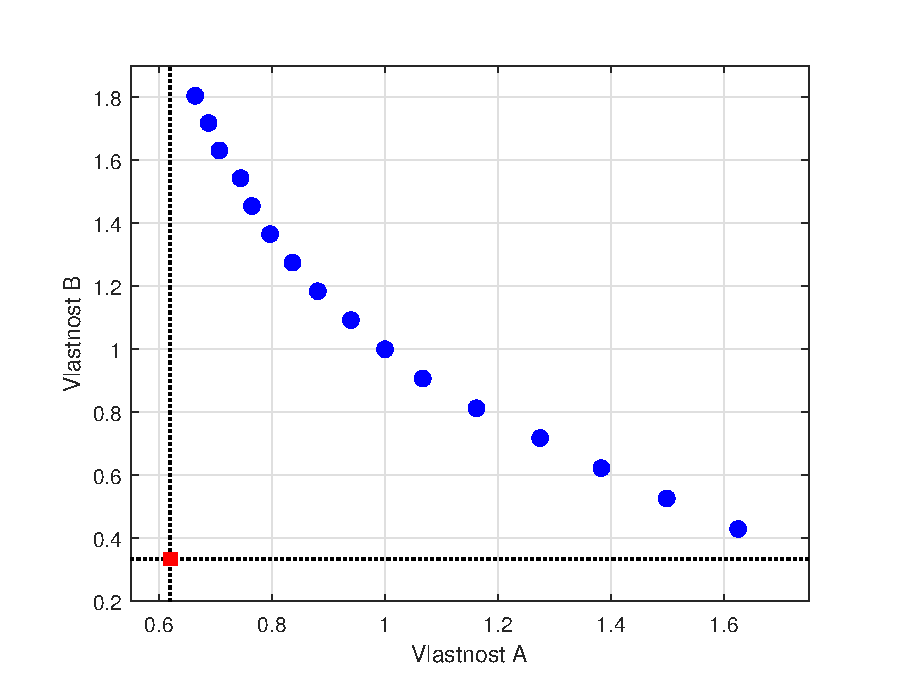
\includegraphics[width=0.7\linewidth]{images/Pareto_ex}
	\caption{Zobrazenie Pareto front -- optimálne riešenia (modrá), utopický bod (červená).}
	\label{fig:Pareto_example}
\end{figure}

Pareto front môžeme využiť aj pri verifikácii kvality dátových modelov. Stačí ak zobrazíme niektoré skúmané vlastnosti vybraného súboru modelov, napríklad presnosť a nadhodnotenie (v zmysle zložitosti modelu, \textit{angl. \aps{overestimation}}), ktoré sa snažíme zlepšiť, optimalizovať. A na základe predchádzajúcej úvahy vyberieme taký model, ktorý bude predstavovať ten najlepší možný kompromis medzi pozorovanou presnosťou modelu a nadhodnotením.
	\section{Identifikácia FIR modelu}
Doteraz sme načrtli situáciu, ako by sme mohli využiť metódu garantovaného odhadu na určenie minimálnej štruktúry modelu a odhad jeho parametrov. Poďme si teraz ukázať ako by sme túto metódu mohli aplikovať na niektorých dátových dynamických modeloch a začneme s FIR modelom.

Najskôr si pripomenieme štruktúru FIR modelu. Ako uvádza rovnica \ref{eq:FIR_m}, FIR model má nasledovný tvar
\begin{equation*}
	\hat{y}(t) = \sum_{i=1}^{n_b} b_{i}u(t-i) = b_{1}u(t-1) + b_{2}u(t-2) + \dots + b_{n_b}u(t-n_b),
\end{equation*}
kde $ n_b $ predstavuje rád modelu, resp. počet parametrov $ b $. 

Aby sme mohli odhadnúť parametre takéhoto modelu, potrebujeme najskôr poznať jeho štruktúru. Na to využijeme metódu odhadu minimálneho rádu modelu, ktorú sme zadefinovali ako \ref{eq:GPE_m_order_est}. V tomto prípade musíme danú formuláciu upraviť do tvaru
\begin{equation}
	\begin{split}
		& \min_{B \in \left[ b_{1}, b_{2}, \dots, b_{n_b} \right]} \quad 0, \\
		& \qquad \quad \text{s.t.} \quad \ubar{e} \leq y - \hat{y} \leq \bar{e}
	\end{split}
	\label{eq:gpe_fir_min_rad}
\end{equation} 
ktorá nám vráti hodnotu minimálneho rádu FIR modelu $ n_b $. V tomto momente už máme k dispozícii informáciu o vyhovujúcej štruktúre modelu, ktorá vyhovuje podmienke GOP. Nasleduje odhad intervalových hodnôt parametrov. Tie získame modifikáciou rovnice \ref{eq:gpe:general_form}
\begin{equation}
	\begin{split}
		\left[ \ubar{b}_i, \bar{b}_i \right] = \min_{B \in \left[ \ubar{b}, \bar{b} \right]} / &\max_{B \in \left[ \ubar{b}, \bar{b} \right]} \quad b_i,\\
		\text{s.t.}& \quad \ubar{e} \leq y - \hat{y} \leq \bar{e}	
	\end{split}
	\label{eq:gpe_fir_param_est}
\end{equation}
pre všetky $ i = 1, 2, \dots, n_b $.  

Týmto sme ukončili identifikáciu FIR modelu minimálneho rádu a v ďalšom postupe by sme sa mali venovať overovaniu správnosti a posudzovaniu kvality daného modelu a modelov vyššieho rádu.

\section{Identifikácia ARX modelu}
ARX model, ako opisuje rovnica \ref{eq:ARX_m}, má štruktúru doplnenú o člen $ A(q) $ oproti FIR modelu a má tvar
\begin{equation*}
	\begin{split}
		\hat{y}(t) &= \frac{\sum_{i=1}^{n_b} b_{i}u(t-i)}{1 + \sum_{i=1}^{n_a} a_{i}q^{-i}} =\\
		&= -a_{1}\hat{y}(t-1) - \dots -a_{n_a}\hat{y}(t-n_a) + b_{1}u(t-1) + \dots + b_{n_b}u(t-n_b).
	\end{split}
\end{equation*}
Výhodou ARX modelu je, že dokáže drasticky znížiť počet parametrov oproti FIR modelu, kvôli príspevku minulých výstupov $ \hat{y}(t-i) $. Avšak, v porovnaní s identifikáciou FIR modelu, je identifikácia ARX modelu omnoho zložitejšia problematika. Práve príspevok minulých výstupov nám transformuje optimalizačnú úlohu z jednoduchej lineárnej (ako to bolo pri identifikácii FIR modelu) na zložitú nelineárnu. V každom prípade postup identifikácie ostáva rovnaký. Najskôr určíme minimálnu štruktúru ARX modelu, ktorá spĺňa podmienky GOP a v ďalšom kroku odhadneme jej parametre resp. intervalové hodnoty parametrov. 

Minimálnu štruktúru ARX modelu, teda rád čitateľa $ n_b $ a rád menovateľa $ n_a $, nájdeme ako riešenie danej optimalizačnej úlohy
\begin{equation}
	\begin{split}
		\min_{a_{1},\dots,a_{n_a},b_{1},\dots,b_{n_b},\hat{y}(t)} & \quad 0.\\
		\text{s.t.} \qquad \quad  & \quad \ubar{e} \leq y - \hat{y} \leq \bar{e} \\
		& \quad \hat{y}(0) = \hat{y}_{0}
	\end{split}
	\label{eq:gpe_arx_min_rad}
\end{equation}
A odhad intervalových hodnôt parametrov určíme ako
\begin{equation}
	\begin{split}
		\left[ \ubar{\theta}_i, \bar{\theta}_i \right] = \min_{\Theta \in \left[ \ubar{\theta}, \bar{\theta} \right]} / \max_{\Theta \in \left[ \ubar{\theta}, \bar{\theta} \right]} & \quad \theta_i,\\
		\text{s.t.} \qquad & \quad \ubar{e} \leq y - \hat{y} \leq \bar{e}\\
		& \quad \hat{y}(0) = \hat{y}_{0}
	\end{split}
	\label{eq:gpe_arx_param_est}
\end{equation}
pre všetky $ i = 1,2, \dots, n_a+n_b $ a $ \Theta $ predstavuje vektor minimálnych a maximálnych hodnôt parametrov $ a, b $
\begin{equation*}
	\Theta = 
	\begin{pmatrix}
		\ubar{a}_{1} & \bar{a}_{1}\\
		\ubar{a}_{2} & \bar{a}_{2}\\
		\vdots & \vdots\\
		\ubar{a}_{n_a} & \bar{a}_{n_a}\\
		\ubar{b}_{1} & \bar{b}_{1}\\
		\ubar{b}_{2} & \bar{b}_{2}\\
		\vdots & \vdots\\
		\ubar{b}_{n_b} & \bar{b}_{n_b}\\	
	\end{pmatrix}.
\end{equation*}
Zložitosť týchto optimalizačných úloh je pravdepodobne očividná. Okrem toho, že nutne musíme v každom nameranom bode odhadovať hodnotu $ \hat{y}(t) $, čo nám pridáva na počte odhadovaných parametrov, tak k nelineárnej optimalizácii potrebujeme pristupovať špeciálne, pretože jej výsledky nemusia konvergovať k spoľahlivému riešeniu.

\section{Príklady identifikácie}
V tejto časti si na konkrétnom príklade ukážeme identifikáciu FIR aj ARX modelu. Začnime tým, že si zadefinujeme problematiku. Predstavme si, že sme z neznámeho procesu získali údaje o vstupoch a výstupoch, tak ako je znázornené na Obr. \ref{fig:gpe_tf_ex_data}, ktoré sú v skutočnosti opísané prenosovou funkciou 1. rádu so zosilnením $ K = 8 $ a časovou konštantou $ T = 2 $
\begin{equation*}
	G(s) = \frac{K}{Ts + 1} = \frac{8}{2s + 1}.
\end{equation*}
Tak ako všetky reálne dáta, výstupné údaje sú zaťažené šumom, a presnosť merania senzora je $ e = \pm 0.8 $. 

\begin{figure}
	\centering
	\begin{subfigure}[b]{0.48\textwidth}
		\centering
		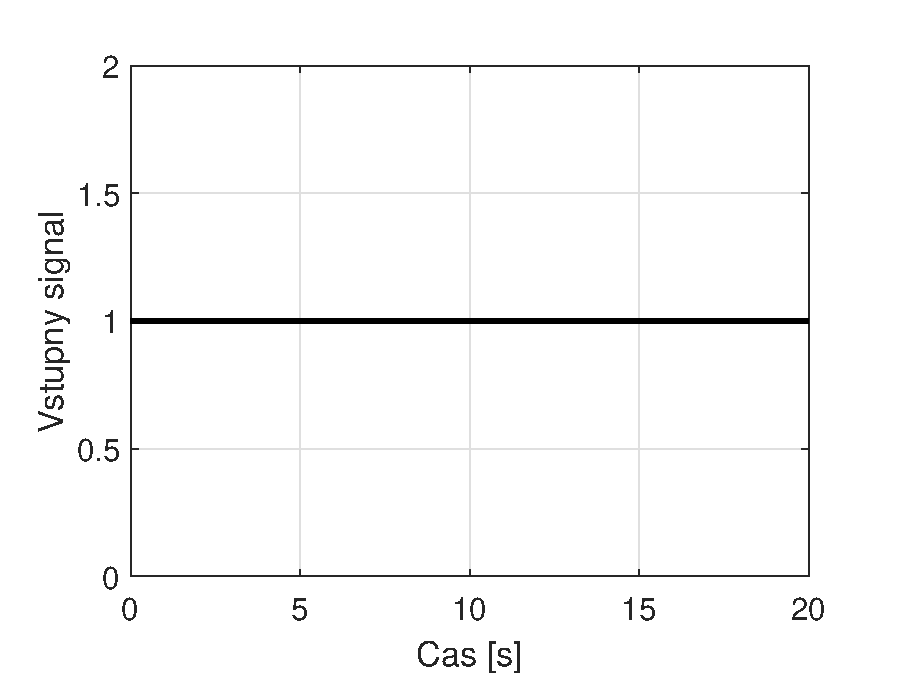
\includegraphics[width=\linewidth]{images/gpe_tf_ex_input}
		\caption{Vstupné údaje}
	\end{subfigure}
	\begin{subfigure}[b]{0.48\textwidth}
		\centering
		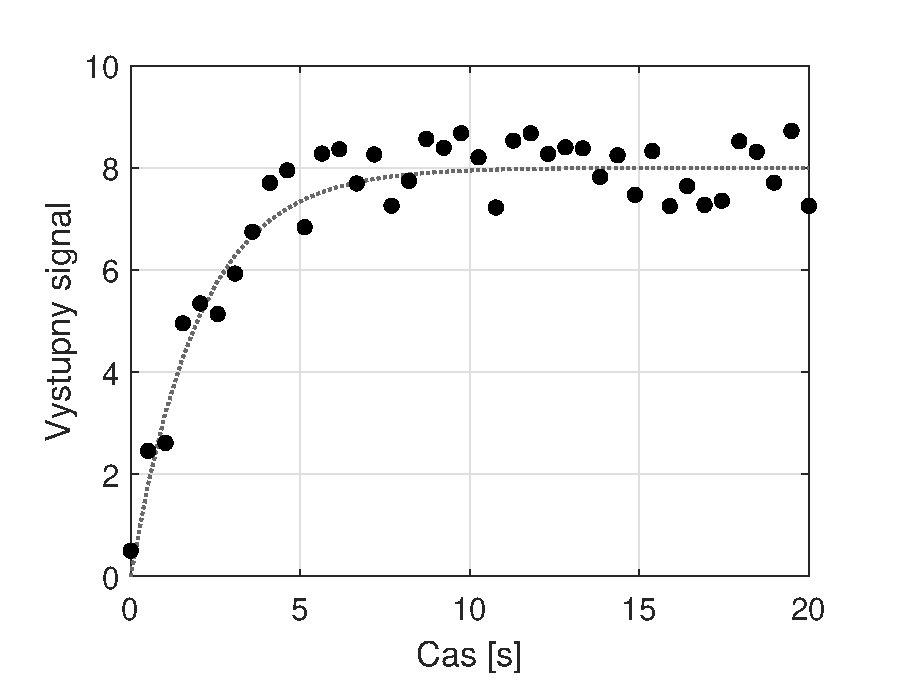
\includegraphics[width=\linewidth]{images/gpe_tf_ex_output}
		\caption{Výstupné údaje}
	\end{subfigure}
	\caption{Namerané dáta z procesu opísaného prenosovou funkciou 1. rádu so zosilnením $ K = 8 $ a časovou konštantou $ T = 2 $.}
	\label{fig:gpe_tf_ex_data}
\end{figure}

Postup identifikácie oboch modelov metódou garantovaného odhadu parametrov je rovnaký. Najskôr odhadneme najjednoduchší model, ktorý vyhovuje podmienke GOP. V prípade FIR modelu môžeme túto problematiku vyjadriť rovnicou \ref{eq:gpe_fir_min_rad} a pre ARX model \ref{eq:gpe_arx_min_rad}. V ďalšom kroku určíme intervalový odhad parametrov danej štruktúry modelu. Riešenie nájdeme podľa rovnice \ref{eq:gpe_fir_param_est}, v prípade FIR alebo podľa \ref{eq:gpe_arx_param_est}, ak sa bude jednať o ARX model.

\begin{figure}
	\centering
	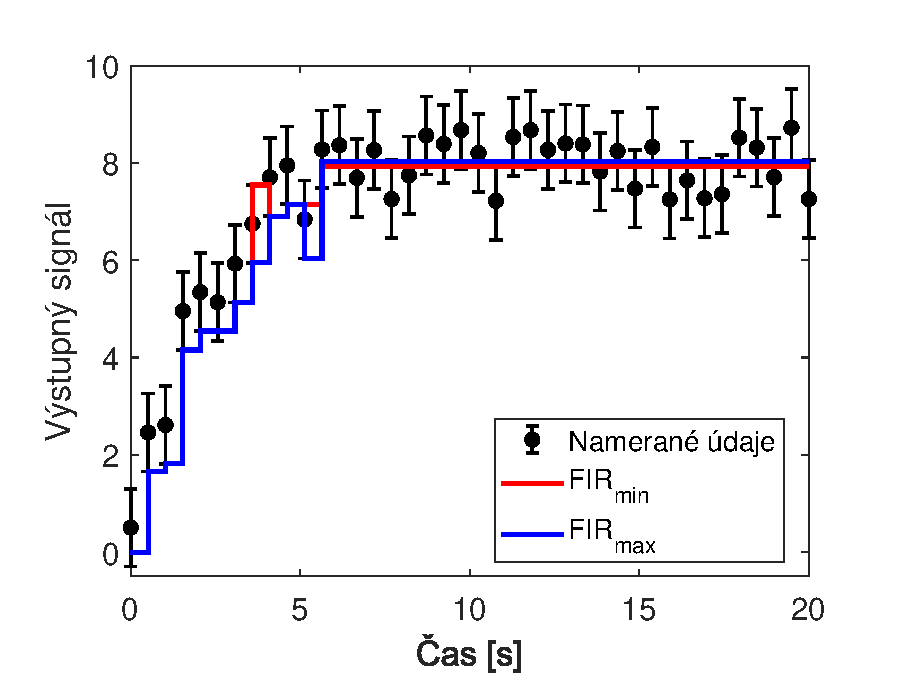
\includegraphics[width=0.7\linewidth]{images/gpe_tf_ex_FIRident}
	\caption{Výsledok identifikácie FIR modelu ($ n_b = 11 $) -- minimálna realizácia (červená), maximálna realizácia (modrá), namerané údaje s danou chybou merania (čierna).}
	\label{fig:gpe_tf_ex_FIR}
\end{figure}

Výsledok identifikácie FIR modelu môžeme vidieť na Obr. \ref{fig:gpe_tf_ex_FIR}. Minimálna veľkosť modelu, ktorá dokázala vhodne opísať dané dáta v stanovej chybe merania, bola $ n_b = 11 $. Po intervalovom odhade parametrov sme získali FIR v nasledovnom tvare
\begin{equation*}
	\begin{split}
		\hat{y}(t) \quad = \quad &[1.6587, 3.2587]u(t-1) + [-1.4459, 1.7541]u(t-2) + \\
		 + &[0.7417, 3.9417]u(t-3) + [-1.2112, 1.9888]u(t-4) + \\
		 + &[-1.8069, 1.3931]u(t-5) + [-0.8084, 2.3916]u(t-6) + \\
		 + &[-0.7821, 2.4179]u(t-7) + [-0.6424, 2.5576]u(t-8) + \\
		 + &[-1.3556, 1.8444]u(t-9) + [-2.7116, 0.4884]u(t-10) + \\
		 + &[0.2836, 1.9842]u(t-11).
	\end{split}
\end{equation*}

Výstup identifikácie ARX modelu môžeme vidieť na Obr. \ref{fig:gpe_tf_ex_ARX}. Minimálna štruktúra bola opísaná diferenčnou rovnicou procesu 1. rádu a po odhade intervalových hodnôt parametrov, sme získali model v tvare
\begin{equation*}
	\hat{y}(t) = [0.7581, 0.7840]\hat{y}(t-1) + [1.7396, 1.9155]u(t-1).
\end{equation*}

\begin{figure}
	\centering
	\psfrag{Cas [s]}{Čas [s]}
	\psfrag{Vystupny signal}{Výstupný signál}
	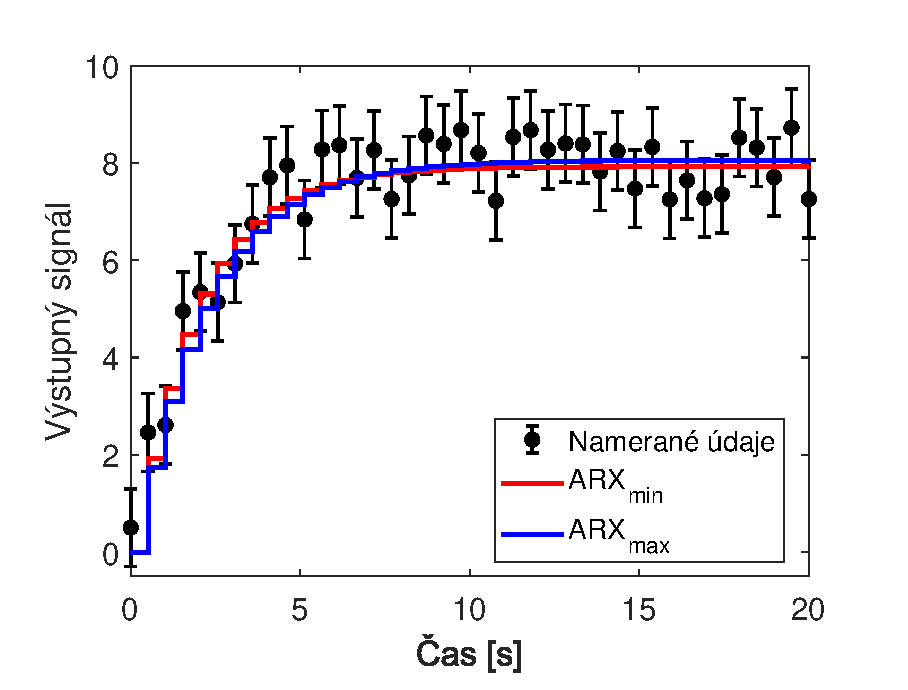
\includegraphics[width=0.7\linewidth]{images/gpe_tf_ex_ARXident}
	\caption{Výsledok identifikácie ARX modelu ($ n_b = 1, n_a = 1 $) -- minimálna realizácia (červená), maximálna realizácia (modrá), namerané údaje s danou chybou merania (čierna).}
	\label{fig:gpe_tf_ex_ARX}
\end{figure}

Rozdiel v zložitosti modelov je očividný, avšak v oboch prípadoch sme získali oblasť riešení, ktorá nám garantuje, že skutočné riešenie leží niekde vo vnútri. Táto oblasť je definovaná kombináciou minimálnych resp. maximálnych parametrov, ktoré nám zabezpečia spodné (minimálna realizácia) resp. horné (maximálna realizácia) ohraničenie. Treba taktiež spomenúť, že nie sme odkázaný iba na intervalový odhad. Akonáhle získame informáciu o štruktúre modelu, môžeme využiť napríklad metódu najmenších štvorcov (MNŠ) na identifikáciu neznámych parametrov. 

	\section{Príklady identifikácie}

	
	% PART 2 - Pouzitie hybridnych modelov
	%hybridne modelovanie
	\part{Hybridné modelovanie a jeho využitie v praxi}
\chapter{Hybridné modelovanie}
Úlohou modelovania procesov je získať matematický predpis na základe znalostí, ktoré o tomto procese máme \cite{hangos:process_modelling:2001}. V závislosti od prístupu k modelovaniu, môžeme získané modely rozdeliť do viacerých skupín. Prvou skupinou sú tak zvané \aps{mechanické} modely. Tieto sú odvodené z fyzikálnych zákonov, ktoré predstavujú rôzne zákony zachovania -- bilancie, hmoty alebo energie, zákony kinetiky, termodynamiky, prestupu látky atď \cite{bangi:chem_engineer:2020}. Takéto modely sú transparentné a ľahko pochopiteľné, pretože majú za sebou skutočnú fyzikálnu podstatu, ktorá platí pre široké spektrum
% RP: Po slovensky je skor "prevadzkovych" ako "operačných"
operačných podmienok. Nevýhodou býva, že často sú veľmi zložité a samotné modelovanie je náročné na čas. Druhú skupinu tvoria dátové modely, ktorých problematiku sme rozobrali v predchádzajúcich kapitolách. Spomenieme, že majú viacero výhod -- sú jednoduché na získanie, čím ušetríme
% RP: "kopec času" je prilis neformalne
kopec času s modelovaním, často majú jednoduchšiu štruktúru, sú flexibilnejšie atď. Nevýhodou však je, že ich štruktúra nám neprezradí nič o samotnej povahe procesu. Hybridné modely tvoria tretiu skupinu a  sú kombináciou mechanických a dátových modelov, pričom využívajú výhody z obidvoch skupín, čím našli široké uplatnenie v rôznych oblastiach -- bioinžinierstvo \cite{srivastava:hybrid_biomolecules:2020}, strojníctvo \cite{liu:hybrid_vehicle:2020}, životné prostredie \cite{liu:hybrid_waste_water:2019}, energetika \cite{qian:hybrid_energy:2019} atď.

\section{Hybridné modely}
Základy hybridného modelovania položili Psichogios a Ungar v práci \aps{\textit{A hybrid neural network-first principles approach to process modeling}} z roku 1992 \cite{psichogios:hybrid_process_model:1992}. Ich cieľom bolo vytvoriť hybridný model založený na neurónovej sieti a mechanickom 
% RP: "modely"
modely vsádzkového biochemického reaktora. Vo výsledku sa im podarilo zlepšiť presnosť predikcie v porovnaní so samotným mechanickým modelom, dosiahnuť lepšiu interpoláciu a extrapoláciu na rozdiel
% RP: "od ... sieti"?
od samotnej neurónovej sieti a výrazne sa uľahčila analýza a interpretácia dát.

Treba zdôrazniť, že pri viacerých chemických, biologických a rôznych ďalších procesoch sú parametre modelu neznáme, pretože zohľadňujú napr. kinetiku konkrétnej chemickej reakcie alebo rast mikroorganizmov, ktorý je špecifický pre konkrétny druh. Ak dátový model dokáže poskytnúť tieto neznáme parametre mechanickému modelu, tak výsledný hybridný model je vhodný aj na predikciu údajov, a tým pádom sa môže využiť na optimalizáciu procesov.

\begin{figure}
	\centering
	% RP: Tu by sa dala zlepsit kvalita sipok, niekore nie su uplne vodorovne.
	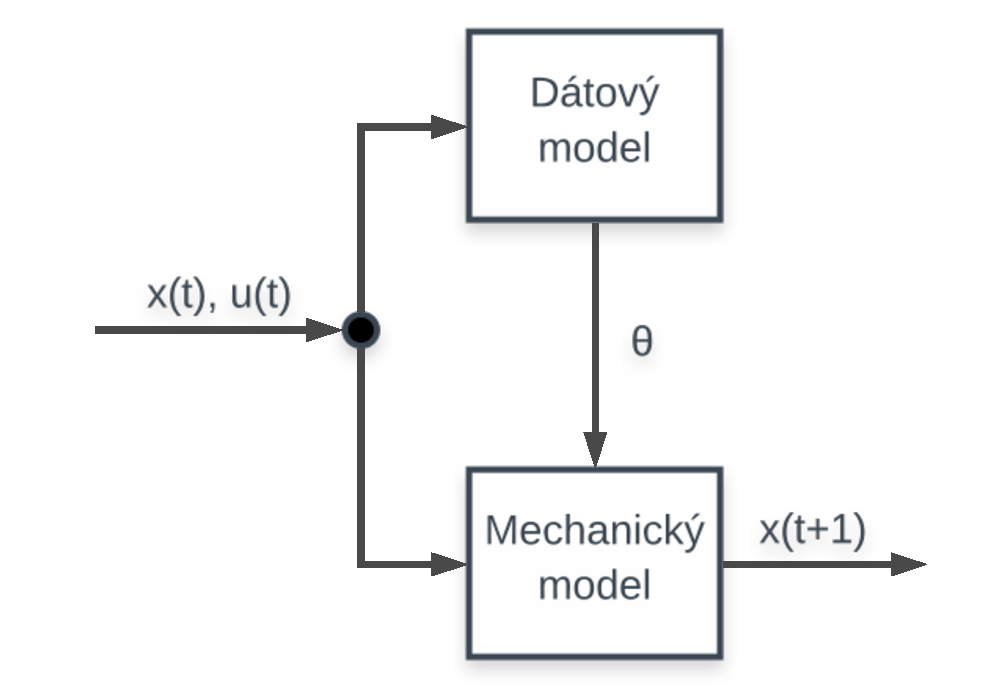
\includegraphics[width=\linewidth]{images/hybrid_model}
	\caption{Architektúra hybridných modelov - a) v sérii, b) paralelne, c) kombinácia v sérii-paralelne.}
	\label{fig:hybrid_model_general}
\end{figure} 

Existuje veľa rôznych kombinácii mechanických a dátových modelov, ktoré vedú k ešte väčšiemu množstvu hybridných modelov, ale vo všeobecnosti by sme mohli sformulovať tri základné štruktúry hybridných modelov, ktoré sú zobrazené na Obr. \ref{fig:hybrid_model_general}.

\textbf{Zapojenie v sérii.} Takáto štruktúra hybridných modelov sa využíva na odhad neznámych  a časovo-premenných kinetických parametrov $ \theta $ \cite{bhutani:hybrid_modelling_opt:2006}.\newline
\textbf{Paralelné zapojenie.} Zatiaľ čo nominálny mechanický model zachytáva správanie systému, dátová časť koriguje rozdiely $ \Delta $ medzi skutočným zariadením a mechanickým modelom. Dátový model natrénovaný na týchto rozdieloch, kompenzuje chyby, ktoré vyplývajú z bežných variácií procesu a nelineárnej komplexnej kinetiky \cite{bhutani:hybrid_modelling_opt:2006}.\newline
\textbf{Kombinovaný prístup -- sériovo-paralelné zapojenie.} V tomto prípade daná architektúra obsahuje dva dátové modely -- jeden, ktorý odhaduje neznáme parametre systému $ \theta $ (v sérii) a druhý, ktorý upravuje výstupy z mechanického modelu o rozdiel oproti skutočnému zariadeniu (paralelne). 

	%ekonomicka optimalizacia
	\section{Optimalizácia prevádzky dynamických systémov}
Optimalizácia je prostriedok, ktorým sa dosiahne najlepší výsledok za daných okolností. Pri navrhovaní, stavbe a údržbe akéhokoľvek inžinierskeho systému, musia inžinieri prijať mnoho technologických a manažérskych rozhodnutí v niekoľkých fázach. Konečným cieľom všetkých takýchto rozhodnutí je buď minimalizovať potrebné úsilie alebo maximalizovať požadovaný úžitok. Pretože úsilie alebo úžitok, požadovaný v akejkoľvek praktickej situácii, môže byť vyjadrený ako funkcia určitých rozhodovacích premenných, optimalizácia môže byť definovaná ako proces hľadania podmienok, ktoré poskytujú maximálnu alebo minimálnu hodnotu funkcie. Na Obr. \ref{fig:cost_fun_ex} môžeme vidieť, že ak bod $ x^{\star} $ zodpovedá minimálnej hodnote funkcie $ f(x) $, rovnaký bod zodpovedá maximálnej hodnote negatívnej hodnote $ -f(x) $ tej istej funkcie. V tom prípade môžeme optimalizáciu bez straty zovšeobecniť na proces minimalizácie, pretože maximum funkcie dokážeme nájsť ako minimum negatívnej hodnoty rovnakej funkcie~\cite{rao:intro_engin_opt:2009}. 

\begin{figure}
	\centering
	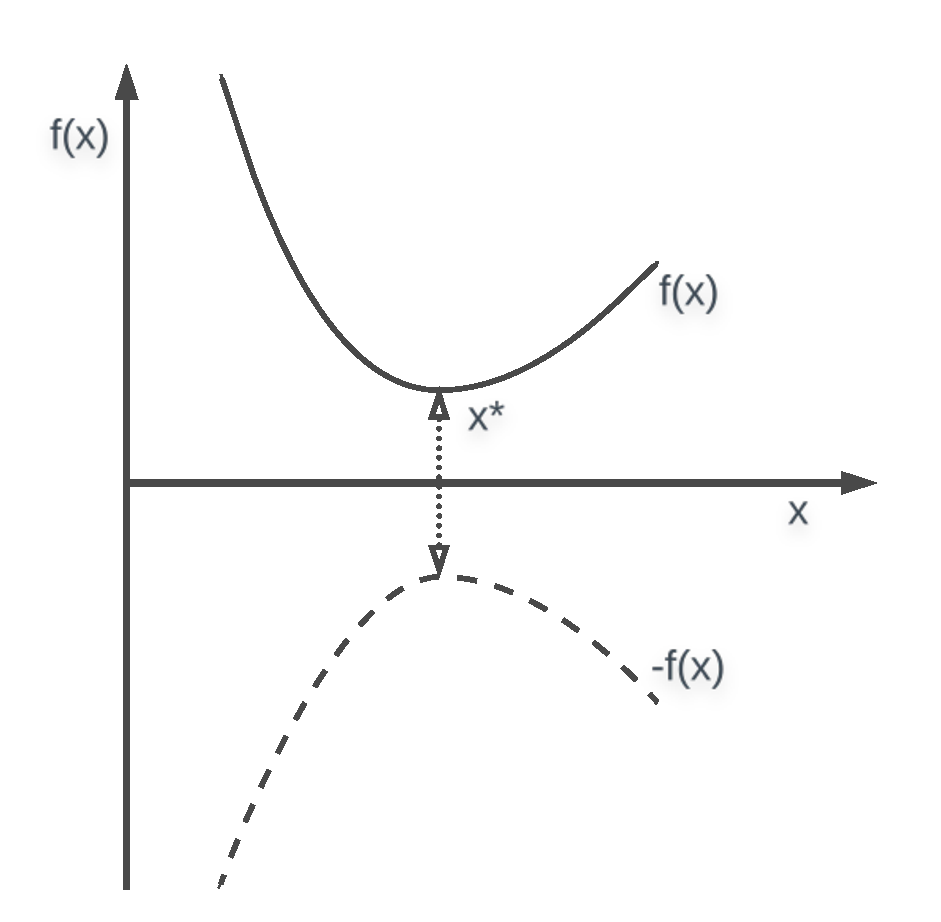
\includegraphics[width=0.5\linewidth]{images/optimization_obj}
	\caption{Minimum účelovej funkcie $ f(x) $ je v rovnakom bode ako maximum $ -f(x) $.}
	\label{fig:cost_fun_ex}
\end{figure}

Pri návrhu optimalizačného problému, môže nastať niekoľko situácii -- (a) v najlepšom prípade získame neohraničenú optimalizačnú úlohu, (b) budeme mať ohraničenia v tvare rovnosti alebo (c) zakomponujeme aj ohraničenia v tvare nerovností. Všetky tieto problémy sa často vyskytujú pri riešení efektivity zariadenia a nazývajú sa problémy statickej~\cite{agrawal:static_opt:1999}. Statická je preto, lebo premenné $ x $ účelovej funkcie $ f(x) $ sú nezávislé od času, nemenia sa. 

Majme všeobecný dynamický systém, ktorý vieme opísať nasledovným modelom
\begin{equation*}
	\der{x}{t} = f(t, x, u, \theta),
\end{equation*}
kde $ x $ sú stavy systému, $ u $ je riadiaca veličina a $ \theta $ predstavuje parametre modelu. Potom ak definujeme účelovú funkciu $ \ell_e(\bar{x},\bar{u}) $, ktorá vyjadruje ekonomickú kvalitu systému, môžeme získať optimálne ustálené stavy $ \bar{x}^{\star}, \bar{u}^{\star} $ ako
\begin{equation}
	\begin{split}
		\min_{\bar{x},\bar{u}}& \quad \ell_e(\bar{x},\bar{u}), \\
		\text{s.t.}& \quad \dot{x} = f(t, x, u, \theta) = 0 \\
		& \quad \bar{x}_{\min} \leq \bar{x} \leq \bar{x}_{\max} \\
		& \quad \bar{u}_{\min} \leq \bar{u} \leq \bar{u}_{\max}
	\end{split}
	\label{eq:econ_opt_dyn_sys}
\end{equation}
ktoré zaručia, že daná účelová funkcia bude dosahovať minimum v danom bode~\cite{hernandez:economics_opt_w_mismatch:2019}. Takýmto spôsobom dokážeme na základe statickej optimalizácie optimalizovať prevádzku akéhokoľvek dynamického systému. Treba však zdôrazniť, že celá táto problematika je založená na poznaní matematického opisu zariadenia. V prípade, že model nebude ekvivalentný so skutočným zariadením (čo v podstate nikdy nie je), získané výsledky nebudú optimálne, v horšom prípade môžu narušiť celé fungovanie zariadenia. To ako sa vysporiadať s touto problematikou vysvetlíme v nasledujúcich častiach.

\subsection{Dvojkroková optimalizácia}
\label{ch:theory_TwoStep}
Dvojkroková optimalizácia je metóda, ktorá pozostáva z dvoch krokov, resp. z dvoch optimalizačných úloh. V prvom kroku, na základe nameraných údajov vstupov $ u $ a stavov $ x $ resp. výstupov $ y $, odhadneme neznáme parametre modelu, ktorý opisuje náš dynamický systém. Túto optimalizačnú úlohu by sme mohli sformulovať podobne ako uvádza rovnica \eqref{eq:param_est_opt_form}. V druhom kroku využijeme informácie z tohto modelu, napr. informácie o ustálených stavoch $ \bar{x} $, na výpočet optimálnych ustálených hodnôt $ \bar{x}^{\star}, \bar{u}^{\star} $, ktoré môžeme aplikovať na naše zariadenie. Takúto problematiku by sme mohli sformulovať ako v prípade \eqref{eq:econ_opt_dyn_sys}. V princípe je možné tento cyklus zopakovať niekoľkokrát, pričom po každom cykle by sme mali získať presnejšie výsledky vzhľadom na daný model.

V skutočnosti táto metóda nerieši problém v rozdiele medzi skutočným zariadením a modelom, i keď v určitých prípadoch dokážeme ladením parametrov modelu zmenšiť tento rozdiel.

\subsection{Schéma úpravy modifikátora}
Najskôr treba uviesť, že ide o metódu, ktorá jednak hľadá optimum prevádzky dynamických systémov a jednak rieši problematiku rozdielu nominálneho modelu od skutočnosti. Okrem iného ide o techniku, ktorá má uplatnenie v dynamickej optimalizácii a v posledných rokoch nadobudla na významnosti~\cite{marchetti:modifier_adapt_scheme:2020}.

Schéma úpravy modifikátora (\textit{angl. \aps{Modifier Adaptation Scheme}}) je iteračná metóda, ktorá ma skvelé uplatnenie v reálnom živote. Hlavnými črtami sú spôsob, akým sa merania používajú na korekciu nominálneho modelu, a úloha, ktorú neskôr model zohráva pri výpočte ďalších vstupov.

Princíp tejto metódy spočíva v úprave gradientu účelovej funkcie nominálneho modelu $ \nabla_N\ell_e(\bar{x},\bar{u}) $ následovným štýlom
\begin{equation}
	\nabla J = \nabla_N\ell_e(\bar{x},\bar{u}) + \lambda_k,
\end{equation}
kde $ \lambda_k $ predstavuje hodnotu modifikátora v $ k $-tom kroku. Upravený gradient po integrácii má tvar 
\begin{equation}
	J^{\tiny{(MA)}} = \ell_e(\bar{x},\bar{u}) + \lambda_ku.
\end{equation}
Hodnota modifikátora v $ k $-tom kroku je určená na základe váhovania dvoch faktorov. Určitú časť prispievajú minulé hodnoty modifikátora $ \lambda_{k-1} $ a zvyšnú časť tvorí rozdiel v gradientoch účelových funkcii $ \Delta_{k-1} $ skutočného zariadenia a nominálneho modelu 
\begin{equation}
	\label{eq:mas_weight}
	\lambda_k = c\lambda_{k-1} + \left(1 - c\right)\Delta_{k},
\end{equation}
kde $ c $ je váhový koeficient, ktorý môže nadobúdať hodnoty $ c \in \lbrace 0; 1 \rbrace $ v závislosti od toho, či chceme aby sa modifikátor menil viac alebo menej s pribúdajúcimi dátami.

Hodnotu premennej $ \Delta_k $ je náročné určiť správne, pretože obsahuje gradient účelovej funkcie reálneho zariadenia $ \nabla_P\ell_e(\bar{x},\bar{u}) $, ktorý my nemáme k dispozícii a preto je nutné ho odhadnúť napr. metódou konečných rozdielov
\begin{equation}
	\nabla_P\ell_{e,k}(\bar{x},\bar{u}) = \frac{\ell_{e,k}(\bar{x},\bar{u}) - \ell_{e,k-1}(\bar{x},\bar{u})}{\bar{u}_k - \bar{u}_{k-1}}.
\end{equation} 
Potom $ \Delta_k $ môžeme definovať ako 
\begin{equation}
	\label{eq:mas_correction}
	\Delta_k = \nabla_P\ell_{e,k}(\bar{x},\bar{u}) - \nabla_N\ell_{e,k}(\bar{x},\bar{u}).
\end{equation}
Treba spomenúť fakt, že práve odhad gradientu účelovej funkcie skutočného zariadenia $ \nabla_P\ell_{e,k}(\bar{x},\bar{u}) $ spôsobuje najväčšie nepresnosti, najmä kvôli šumu merania. 

\subsection{Použitie hybridných modelov}
Hybridné modelovanie si takisto dokáže poradiť s optimalizáciou prevádzky, pričom jasnou výhodou je, že nepotrebuje odhadovať gradient účelovej funkcie, ktorý prispieva najväčšou neistotou metóde úpravy modifikátora. V niektorých vedeckých publikáciach sa ukázalo, že využitie hybridných modelov, pri optimalizácii prevádzky dynamických systémov, výrazne dopomohlo k zvýšeniu efektivity, najmä kvôli lepším predikčným vlastnostiam hybridných modelov~\cite{bhutani:hybrid_modelling_opt:2006}. 

Pri zostavovaní optimalizačnej úlohy musíme dbať na funkčnosť hybridného modelu. V prípade sériového zapojenia by táto optimalizačná úloha mohla vyzerať nasledovne
\begin{equation}
	\begin{split}
		\min_{\bar{x},\bar{u}} &\quad \ell_e\left(\bar{x},\bar{u}\right).\\
		\text{s.t.} &\quad \dot{x} = f\left(t,x,u,\theta\right) = 0\\
		&\quad \theta = g(u)
	\end{split}
\end{equation}
Dátový model $ g(u) $, ktorý bol vopred natrénovaný na dátach zo zariadenia, odhaduje parametre systému $ \theta $ na základe meniacej sa vstupnej veličiny $ u $. Odhadnuté parametre dopĺňajú nominálny mechanistický model $ f(t,x,u,\theta) $, ktorý poskytuje údaje o ustálených stavoch $ \bar{x} $ v účelovej funkcii $ \ell_e\left(\bar{x},\bar{u}\right) $. 

Paralelné zapojenie je trošku odlišné. Jednak vychádza z predpokladu, že nominálny model, ktorý máme je už identifikovaný. Tým pádom dokážeme získať údaje o rozdieloch $ \Delta $ medzi výstupmi zo skutočného zariadenia a nominálneho modelu. Ná týchto dátach je natrénovaný dátový model $ h^{(1)}(u) $, ktorý na základe vstupných údajov $ u $ upravuje výstupy ustálených stavov $ \bar{x} $ z mechanistického modelu $ f(t,x,u) $. Optimalizačnú úlohu by sme mohli sformulovať ako
\begin{equation}
	\begin{split}
		\min_{\hat{x},\bar{u}} &\quad \ell_e\left(\hat{x},\bar{u}\right),\\
		\text{s.t.} &\quad \dot{x} = f\left(t,x,u\right) = 0\\
		&\quad \hat{x} = \bar{x} + \Delta\\
		&\quad \Delta = h^{(1)}(u)
	\end{split}
\end{equation}
kde $ \hat{x} $ predstavuje upravené ustálené stavy z hybridného modelu.

Sériovo--paralelná štruktúra je akousi kombináciou oboch predchádzajúcich architektúr a optimálne ustálené hodnoty $ \bar{x}^{\star}, \bar{u}^{\star} $ môžeme získať vyriešením  optimalizačnej úlohy v tvare
\begin{equation}
	\begin{split}
		\min_{\hat{x},\bar{u}} &\quad \ell_e\left(\hat{x},\bar{u}\right).\\
		\text{s.t.} &\quad \dot{x} = f\left(t,x,u,\theta\right) = 0\\
		&\quad \theta = g(u) \\
		&\quad \hat{x} = \bar{x} + \Delta \\
		&\quad \Delta = h^{(2)}(u)
	\end{split}
\end{equation}
Treba však zdôrazniť, že dátový model paralelného zapojenia $ h^{(1)} $ nie je totožný s dátovým modelom $ h^{(2)} $ kombinovaného zapojenia, pretože v tomto usporiadaní sú dáta o rozdieloch $ \Delta $ odlišné. Je to spôsobené najmä kvôli meniacim sa parametrom $ \theta $ mechanistického modelu, ktoré sú odhadované druhým dátovým modelom $ g(u) $. Na druhej strane, dátový model $ g(u) $ môže byť rovnaký ako v sériovom zapojení a často aj býva rovnaký. 

	%biochem reaktor
	\section{Optimalizácia biochemického reaktora}
V tejto časti sa budeme venovať, ako už napovedá aj samotný názov, ekonomickej optimalizácii konkrétneho dynamického systému a to prietokového biochemického reaktora. Prečo ? Je na to niekoľko dôvodov. V prvom rade sa biochemické reaktory považujú za dôležitú súčasť chemického priemyslu. Široká škála dôležitých zlúčenín ako farmaceutické produkty, rôzne polyméry alebo produkty potravinárskeho priemyslu sa vyrábajú pomocou určitého fermentačného média (rôzne baktérie, kvasinky, vláknité huby alebo enzýmy) za prísne stanovených podmienok v biochemickom reaktore \cite{srinivasan:chemostat_opt:2003}. V druhom rade, biochemické reaktory vykazujú širokú škálu dynamického správania a ponúkajú veľa problémov s modelovaním v dôsledku prítomnosti živých organizmov (mikroorganizmov), ktorých rýchlosť rastu je opísaná komplexnými kinetickými výrazmi \cite{psichogios:hybrid_process_model:1992}. A v neposlednom rade, optimalizácia prietokového biochemického reaktora je aj jedným z hlavných cieľov tejto práce.

\subsection{Biochemický reaktor - Základné informácie}
Biochemický reaktor sa dá vo všeobecnosti definovať ako nádoba, ktorá využíva aktivitu biologického katalyzátora na dosiahnutie požadovanej chemickej premeny \cite{kaushik:bioreactors:2014}.
Biochemický reaktor všeobecne poskytuje biomechanické a biochemické prostredie, ktoré riadi prenos živín a kyslíka do buniek a produkty metabolizmu z buniek. Dal by sa tiež označiť ako zariadenie, určené na optimálny rast a metabolickú aktivitu organizmu, pôsobením biokatalyzátora, enzýmu alebo mikroorganizmov a buniek zvierat alebo rastlín. Surovinou môže byť organická alebo anorganická chemická zlúčenina alebo dokonca komplexný materiál. Produkt konverzie môže zahŕňať pekárske kvasinky, proteín, štartovacie kultúry alebo primárne metabolity (napr. aminokyseliny, organické kyseliny, vitamíny, polysacharidy, etanol atď.) a sekundárne metabolity (napr. antibiotiká). Biochemické reaktory sa môžu použiť na biokonverziu alebo biotransformáciu produktov (steroidná biotransformácia, L-sorbitol), enzýmov (amyláza, lipáza, celuláza), rekombinantných produktov (niektoré vakcíny, hormóny, ako je inzulín a rastové hormóny). Biochemický reaktor musí byť navrhnutý tak, aby vyhovoval konkrétnemu procesu \cite{kaushik:bioreactors:2014}.

\subsubsection{Rozdelenie biochemických reaktorov}
Na základe spôsobu prevádzky môže byť biochemický reaktor klasifikovaný ako vsádzkový, kontinuálny a polovsádzkový.
 
Pri vsádzkovom spôsobe sa sterilné kultivačné médium naočkuje mikroorganizmami. Počas tohto reakčného obdobia sa s časom menia množstvá buniek, substrátu vrátane výživných solí, vitamínov a produktov. Fermentácia prebieha vopred stanovenú dobu a produkt sa zozbiera na konci.

V polovsádzkovom režime sa do reaktora postupne pridávajú živiny, ako prebiehajú biochemické reakcie, aby sa získali lepšie výťažky a vyššia selektivita spolu s reguláciou reakčnej teploty. Produkty sa zbierajú na konci výrobného cyklu ako pri vsádzkovom biochemickom reaktore. Charakteristickou črtou kontinuálneho biochemického reaktora je proces neustáleho dodávania substrátu. Prúd kvapaliny alebo suspenzie sa kontinuálne privádza a odstraňuje z reaktora. Na dosiahnutie rovnomerného zloženia a teploty je potrebné mechanické alebo hydraulické miešanie. Kultivačné médium, ktoré je buď sterilné alebo obsahuje mikroorganizmy, sa nepretržite dodáva do biochemického reaktora, aby sa udržal stabilný stav. Reakčné premenné a kontrolné parametre zostávajú konzistentné a vytvárajú v reaktore časovo konštantný stav. Výsledkom je nepretržitá produktivita.

Tradičné vsádzkové miešacie tankové reaktory (STR) a kontinuálne miešané tankové reaktory (CSTR) existujú už po stáročia a sú stále široko prijímané v chemickom a biologickom priemysle kvôli ich jednoduchosti. Ostatné biochemické reaktory, ktoré majú špeciálne konštrukčné a prevádzkové vlastnosti sú foto-bioreaktory, rotačné bubnové reaktory, hmlový, membránový biochemický reaktor, reaktory s náplňou a fluidnou vrstvou atď. Tieto boli navrhnuté tak, aby vyhovovali špecifickým procesom \cite{kaushik:bioreactors:2014}.

\subsubsection{Parametre opisujúce biochemický reaktor}
Hlavné premenné, ktoré opisujú mikrobiálne procesy v prírode sú uvedené v Tabuľke \ref{tab:chemostat_dyn_param}.

\textbf{Množstvo mikroorganizmov} môže byť vyjadrené ako biomasa $x$ alebo počet buniek $N$ pri jednobunkových organizmoch (baktérie, kvasinky, spóry) na jednotku pôdy, množstva vody, objemu alebo obsahu plochy. Vláknité organizmy (huby, aktinomycéty) sú charakterizované dĺžkou mycélia $L$ a počtom hýf $n$. Treba zdôrazniť, že $n$ nie je totožné s $N$, pretože vetvenie hýf skôr pripomína delenie buniek pri jednobunkových organizmoch. Vzťah medzi $x$, $N$ a $L$ nie je jednoznačný pretože hmota jednotlivých buniek a šírka hýf sa líši v závislosti od organizmu a podmienok rastu. Všeobecne možno povedať, že pri nadbytku výživných zlúčenín sa formujú veľké bunky resp. široké hýfy, zatiaľ čo pri hladovaní sa tvoria skôr menšie bunky alebo užšie hýfy. Výber biomasy $x$ alebo počet buniek $N$ alebo dĺžku mycélia $L$ závisí na danom prípade. Biomasa $x$ má očividnú výhodu pri skúmaní cyklu uhlíka a živín, zatiaľ čo počet buniek $N$ sa preferuje pri skúmaní populácie napr. výskyt mutácií alebo prenos plazmidov \cite{panikov:kinetics_MO_processes:2016}.

\begin{table}
	\centering
	\caption{Prehľad hlavných dynamických parametrov opisujúcich biochemický reaktor \cite{panikov:kinetics_MO_processes:2016}.}
	\label{tab:chemostat_dyn_param}
	\begin{tabular}{p{5cm} p{1.9cm} p{4cm}}
		\hline
		\textbf{Parameter} & \textbf{Symbol} & \textbf{Rozmer} \\ 
		\hline
		Hustota/koncentrácia biomasy & $x$ & \si{\micro\gram} bunkovej hmoty na \si{\gram} pôdy; \si{\gram} bunkovej hmoty \si{\per\square\meter} pôdy; \si{\micro\gram} bunkovej hmoty na \si{\milli\liter} vody\\
		Počet buniek & $N$ & $10^{6}$ buniek na \si{\gram} pôdy; $10^{6}$ buniek na \si{\milli\liter} vody\\
		Dĺžka mycélia & $ L $ & \si{\meter} na \si{\gram} pôdy; \si{\meter} na \si{\milli\liter} vody\\
		Počet hýf & $n$ & $10^{6}$ na \si{\gram} pôdy; $10^{6}$ na \si{\milli\liter} vody\\
		Koncentrácia limitujúceho substrátu & $s$ & \si{\milli\gram} na \si{\gram} pôdy; \si{\gram\per\square\meter} pôdy; \si{\gram\per\liter}vody\\
		Koncentrácia produktu & $p$ & \si{\milli\gram} na \si{\gram} pôdy; \si{\gram\per\square\meter} pôdy; \si{\gram\per\liter}vody\\
		\hline	
	\end{tabular}
\end{table}

\textbf{Koncentrácia limitujúceho substrátu} vo vode alebo v pôde, $(s)$, predstavuje množstvo esenciálnej živiny využívanej mikroorganizmami na rast a rozmnožovanie. Bežne nevieme posúdiť všetky potenciálne dostupné živiny a zamerať sa iba na jednu alebo zopár individuálnych zlúčenín alebo triedu molekúl, ktorá reprezentuje limitujúcu zlúčeninu, pretože chemoorganotrofné mikroorganizmy čerpajú energiu z organických zlúčenín, zatiaľ čo fotosyntetizujúce mikroorganizmy vyžadujú prísun svetla a zdroj fosforu, dusíka a železa \cite{panikov:kinetics_MO_processes:2016}.

\textbf{Množstvo produktov} $(p)$. Sem patria všetky medziprodukty a konečné produkty metabolizmu mikroorganizmov, ktoré vznikajú počas rastu. Typickými medziproduktmi sú organické kyseliny vznikajúce počas glykolýzy. Jediný konečný produkt aeróbnej mikrobiálnej dekompozície je oxid uhličitý, avšak pri anaeróbnych podmienkach vznikajú rôzne organické kyseliny, alkoholy, ketóny atď. \cite{panikov:kinetics_MO_processes:2016}.
	\section{Matematické modelovanie zariadenia}
Najjednoduchším matematickým modelom, ktorý opisuje prietokový biochemický reaktor je tzv. Monod model. Tento model je veľmi obľúbený hlavne kvôli svojej jednoduchosti. Zakladá sa na dvoch predpokladoch: \text{1)} špecifická rýchlosť rastu buniek závisí od koncentrácie substrátu a \text{2)} tvorba biomasy je spojená so spotrebou substrátu. Formulácia rovníc, ktoré popisujú materiálovú bilanciu biomasy je nasledovná
% RP: Ja by som toto riesil skor cez rovnicove prostredia (pride mi ze za table je prilis velka medzera). Nebolo by zle ani jednotlive cleny ozatvorkovat na zlepsenie citatelnosti.
\begin{table}[H]
	\centering
	\begin{tabular}{ccccc}
		akumulácia & & množstvo & & množstvo \\
		bunkovej & = & vzniknutých & -- & odobraných \\
		hmoty & & buniek & & buniek \\
	\end{tabular}
\end{table}
a pre materiálovú bilanciu substrátu platí:
\begin{table}[H]
	\centering
	\begin{tabular}{ccccccc}
		akumulácia & & množstvo & & množstvo & & množstvo\\
		substrátu & = & dodaného & -- & odobraného & -- & spotrebovaného .\\
		v systéme & & substrátu & & substrátu & & substrátu MO\\
	\end{tabular}
\end{table}
Ak uvažujeme, že objem reaktora sa nemení a prítok substrátu sa rovná odtoku suspenzie, potom môžme písať
% RP: Vsetky premenne treba definovat. V? \mu? Y? Nestaci ak sa toto objavi zrazu o 5 riadkov nizsie.
% RP: Zisiel by sa tu aj odkaz na literaturu.
\begin{align}
	&V\left(\der{x}{t}\right) = V\mu(s)x - Fx, \label{eq:tmp_monod_biomass} \\
	&V\left(\der{s}{t}\right) = Fs_{in} - Fs - V\frac{1}{Y_{x}}\mu(s)x. \label{eq:tmp_monod_subs}
\end{align}
Obe strany rovníc vydelíme objemom reaktora a označíme si pomer $ F/V = D $ ako rýchlosť riedenia, môžeme rovnice \eqref{eq:tmp_monod_biomass} a \eqref{eq:tmp_monod_subs} upraviť do nasledovného tvaru
\begin{align} 
	&\der{x}{t} = \left(\mu(s) - D\right)x, \text{kde}  \qquad \mu(s) = \mu_{m}\frac{s}{K_{M} + s}, \label{eq:monod_biomas}\\
	&\der{s}{t} = D\left(s_{in} - s\right) - \frac{1}{Y_{x}}\mu(s)x. \label{eq:monod_subs}
\end{align}

\subsection{Základné mechanické modely biochemického reaktora}
Rovnice \eqref{eq:monod_biomas} a \eqref{eq:monod_subs} tvoria najjednoduchší opis biochemického reaktora -- Monod model, a význam jednotlivých parametrov je uvedený v Tabuľke \ref{tab:monod_params}. Avšak, tento model má množstvo nedostatkov. Nedokáže vysvetliť jednotlivé fázy rastu, ktoré sú pozorované experimentálne a to: lag-fázu, smrť buniek na základe hladovania, tvorbu produktu atď. Tieto nedostatky boli doplnené u tzv. štrukturovaných modelov. Model, ktorý berie do úvahy aj tvorbu produktu, získame doplnením Monod modelu
\begin{align} 
&\der{x}{t} = \left(\mu(s) - D\right)x, \label{eq:chemostat_biomass}\\
&\der{s}{t} = D\left(s_{in} - s\right) - \frac{1}{Y_{x}}\mu(s)x - \frac{1}{Y_{p}}\nu x, \label{eq:chemostat_substrate}\\
&\der{p}{t} = \nu x - Dp, \label{eq:monod_product}
\end{align}
kde $p$ predstavuje koncentráciu produktu v \si{\gram\per\liter}, $Y_{p}$ je bezrozmerový koeficient výťažnosti produktu a $\nu$ predstavuje kinetický člen rýchlosti tvorby produktu v jednotkách času napr. \si{\per\hour}. Do rovnice \eqref{eq:monod_subs} sme doplnili časť, ktorá vraví, že časť substrátu sa spotrebuje na tvorbu produktu a rovnica \eqref{eq:monod_product} predstavuje obyčajnú materiálovú bilanciu produktu. 

\begin{table}
	\centering
	\caption{Parametre Monod modelu, ich symbol a rozmer.}
	\label{tab:monod_params}
	\begin{tabular}{lll}
		\hline
		\textbf{Parameter} & \textbf{Symbol} & \textbf{Rozmer} \\
		\hline
		Špecifická rýchlosť rastu & $\mu(s)$ & \si{\per\hour} \\
		Maximálna špecifická rýchlosť rastu & $\mu_{m}$ & \si{\per\hour} \\
		Michaelisova konštanta & $K_{M}$ & \si{\gram\per\liter} \\
		Výťažok (biomasa) & $Y_{x}$ & \\
		Objem reaktora & $V$ & \si{\liter} \\
		Prietok substrátu/suspenzie & $F$ & \si{\liter\per\hour} \\
		Koncentrácia biomasy & $x$ & \si{\gram\per\liter} \\
		Koncentrácia substrátu & $s$ & \si{\gram\per\liter} \\
		Koncentrácia čerstvého substrátu & $s_{in}$ & \si{\gram\per\liter} \\
		\hline
	\end{tabular}
\end{table}

Ak by sme chceli do modelu zakomponovať tendenciu úmrtia mikroorganizmov v dôsledku príliš vysokej koncentrácie substrátu (vplyv osmotického tlaku), treba upraviť špecifickú rýchlosť rastu $\mu(s)$ tak, že bude obsahovať inhibičný člen $ K_I $, ktorého rozmer je \si{\gram\per\liter}. Špecifická rýchlosť rastu potom nadobudne tvar
\begin{equation}
\mu(s) = \mu_{m}\frac{s}{K_{M} + s + \frac{s^2}{K_I}} \label{eq:spec_growth_rate_Haldane}
\end{equation}
a model, ktorého špecifická rýchlosť rastu má takéto vlastnosti, sa zvykne nazývať inhibičný alebo tiež Haldane model. 

	\section{Analýza matematických modelov}
V predchádzajúcej časti sme spomenuli viacero modelov, ktorými môžeme opísať biochemický reaktor. V tejto časti sa budeme venovať analýze dynamiky a stability dvoch modelov a to Monod modelu doplnenému o produktovú časť a Haldane modelu.

\subsection{Dynamika}
Matematický model, ktorý opisuje biochemický reaktor je nelineárny model. To znamená, že odozva systému je rôzna pre rovnakú veľkosť skokovej zmeny pri rôznych začiatočných podmienkach. Túto nelinearitu si možno všimnúť na Obr. \ref{fig:dyn_monod_ex}. Ten opisuje časový priebeh koncentrácie biomasy, substrátu a produktu Monod modelu pri viacerých skokových zmenách v rýchlosti riedenia. Ďalej si môžeme všimnúť prudký nárast koncentrácie produktu na počiatku, ktorý bol spôsobený nadbytkom biomasy v systéme. Po ustálení dynamika produktu pripomína systém 1. rádu. Na druhej strane v dynamike tvorby biomasy sa prejavuje nestabilná nula (menšie podkmity), ktoré sú spôsobené v dôsledku zvýšenia prietoku látky cez reaktor. Keďže pritečie viac substrátu, čím sa zvýši jeho koncentrácia, koncentrácia biomasy naopak klesne, keďže odtečie viac suspenzie. Následne zvýšená koncentrácia substrátu podporí rast biomasy a tým sa aj koncentrácia biomasy začne zvyšovať. V dynamike substrátu sa zasa prejavuje stabilná nula, ktorá opäť súvisí s väčším prítokom čerstvého média a pomalšou spotrebou substrátu na tvorbu biomasy a produktu.
\begin{figure}
	\centering
	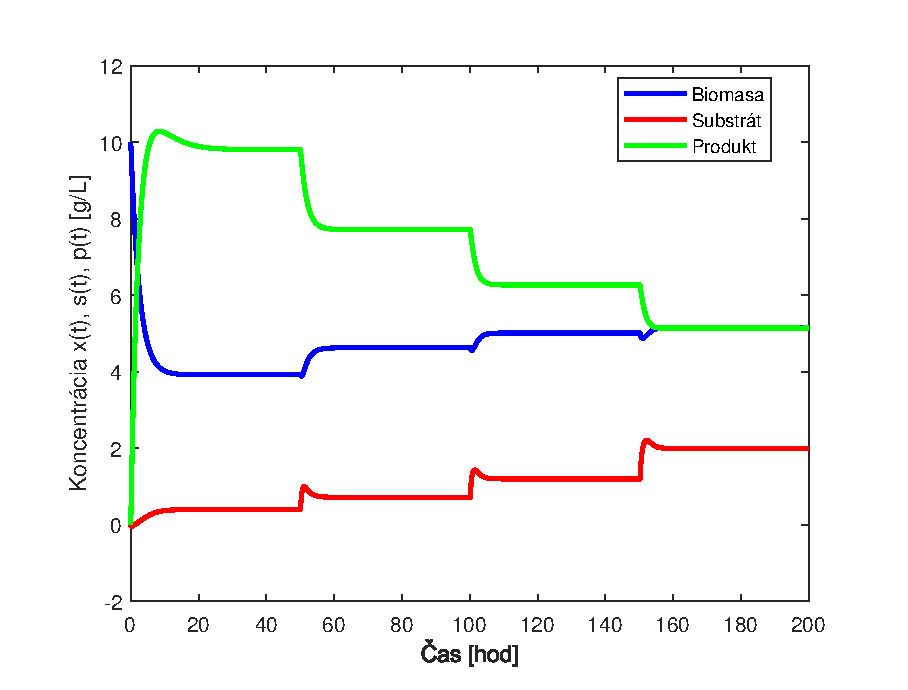
\includegraphics[width=0.7\linewidth]{images/monod_data}
	\caption{Časový priebeh koncentrácie biomasy $ x(t) $, substrátu $ s(t) $ a produktu $ p(t) $ Monod modelu pri viacnásobnej skokovej zmene rýchlosti riedenia $ D = [0.2, 0.3, 0.4, 0.5] $. Parametre modelu: $ \mu_{m} = 0.8\si{\per\hour}, \nu = 0.5\si{\per\hour}, K_{M} = 1.2\si{\gram\per\liter}, Y_{x} = 0.4, Y_{p} = 1, s_{in} = 20\si{\gram\per\liter}, s_0 = p_0 = 0\si{\gram\per\liter} a x_0 = 10\si{\gram\per\liter}$.}
	\label{fig:dyn_monod_ex}
\end{figure}

Režim fungovania biochemického reaktora má významný vplyv na dynamiku celého systému a pri určitých podmienkach Monod model a model s inhibíciou môžu vykazovať rovnaké správanie. Avšak, pri nesprávne zvolených pracovných podmienkach, či už počiatočných podmienkach systému, koncentrácie čerstvého substrátu alebo rýchlosti riedenia, model s inhibíciou bude vykazovať diametrálne odlišné správanie od Monod modelu, ako to je zobrazené na Obr. \ref{fig:dyn_comparison}. Ako môžeme vidieť, zatiaľ čo Monod model sa dostal do nenulového ustáleného stavu, model s inhibíciou klesol s koncentráciou biomasy a produktu na nulu, zatiaľ čo koncentrácia substrátu stúpla na hodnotu 20\si{\gram\per\liter}. Tento stav, kedy reaktorom preteká čistý substrát sa nazýva stav \aps{vymytia} alebo \aps{výplach} a prevádzka reaktora je nenávratne narušená.
\begin{figure}
	\centering
	\begin{subfigure}[b]{0.49\textwidth}
		\centering
		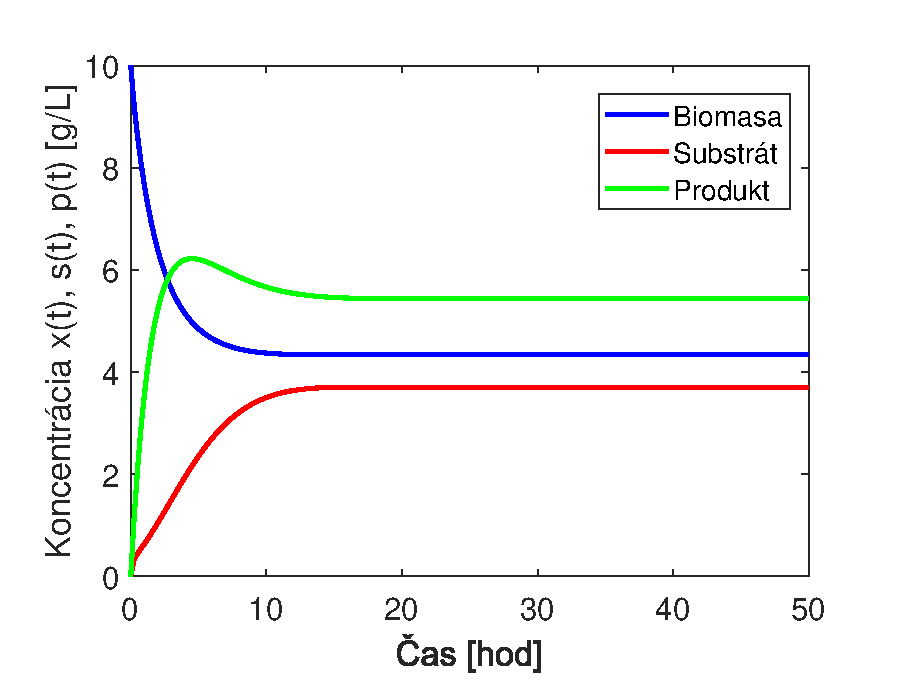
\includegraphics[width=\linewidth]{images/comparison_monod}
		\caption{Monod model}
		\label{fig:dyn_comparison_monod}
	\end{subfigure}
		\begin{subfigure}[b]{0.49\textwidth}
		\centering
		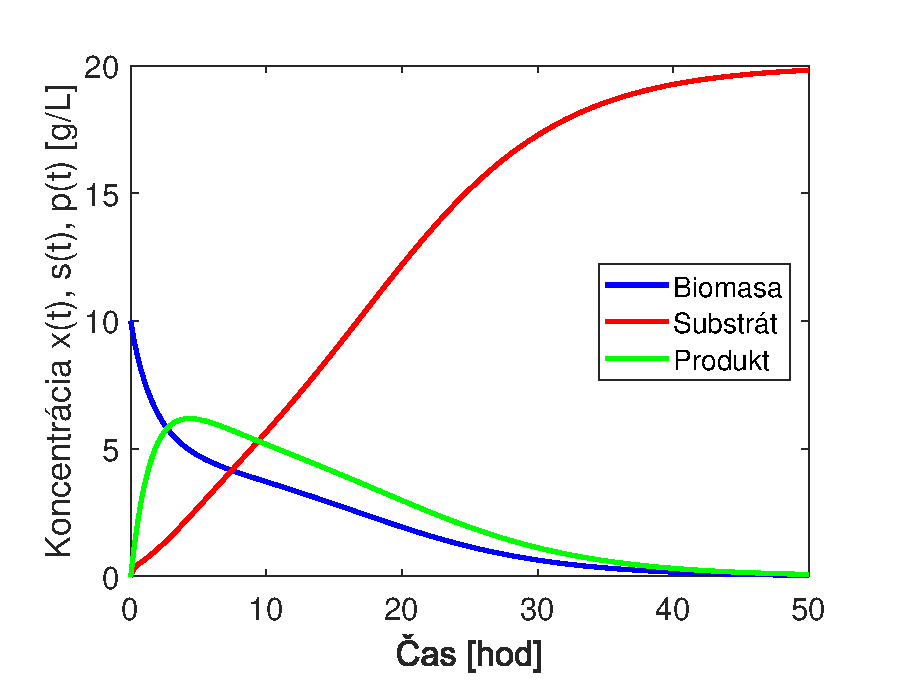
\includegraphics[width=\linewidth]{images/comparison_haldane}
		\caption{Haldane model}
		\label{fig:dyn_comparison_haldane}
	\end{subfigure}
	\caption{Porovnanie dynamiky modelov pri rovnakých pracovných podmienkach. Parametre modelov: $ \mu_{m} = 0.8\si{\per\hour}, \nu = 0.5\si{\per\hour}, K_{M} = 1.2\si{\gram\per\liter}, K_{I} = 20\si{\gram\per\liter}, Y_{x} = 0.4, Y_{p} = 1, s_{in} = 20\si{\gram\per\liter}, s_0 = p_0 = 0\si{\gram\per\liter} a x_0 = 10\si{\gram\per\liter}$.}
	\label{fig:dyn_comparison}
\end{figure}

\subsection{Stabilita}
Výhodou prietokových biochemických reaktorov je, že pri dodržaní správnych podmienok, dokážeme systém uviesť do časovo konštantného stavu. Z rovnice \eqref{eq:monod_biomas} vyplýva, že na dosiahnutie ustáleného stavu, je nutné, aby sa buď špecifická rýchlosť rastu rovnala rýchlosti riedenia (takto získame netriviálne riešenie), alebo koncentrácia biomasy je v ľubovolnom čase rovná nule (takto získame triviálne riešenie -- stav vymytia). Ustálené stavy modelov môžeme vidieť na Obr. \ref{fig:spec_rychl_rastu}, ktorý zobrazuje priebeh špecifickej rýchlosti rastu od koncentrácie substrátu pri konštantnej rýchlosti riedenia. Je dobré si všimnúť, že zatiaľ čo Monod model má iba jeden nenulový ustálený stav, model s inhibíciou už obsahuje dva.
\begin{figure}
	\centering
	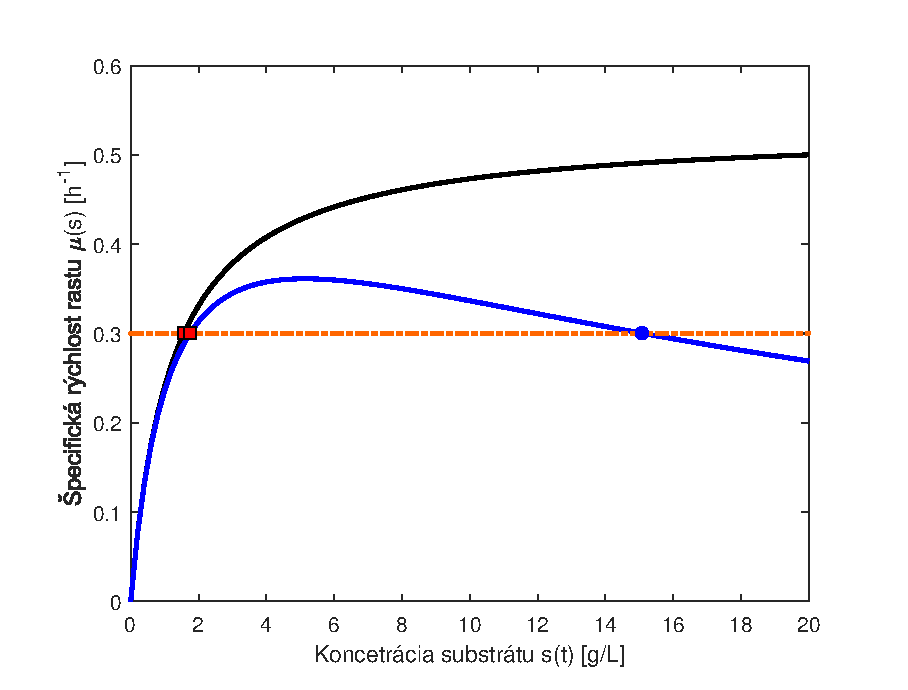
\includegraphics[width=0.7\linewidth]{images/spec_growth_rate}
	\caption{Porovnanie priebehu špecifickej rýchlosti rastu Monod (čierna) a Haldane (modrá) modelu. Zvolená rýchlosť riedenia $ D = 0.33\si{\per\hour} $ (oranžová), stabilné ustálené stavy (červený štvorec), nestabilný stav (modrý krúžok).}
	\label{fig:spec_rychl_rastu}
\end{figure}

\begin{figure}
	\centering
	\begin{subfigure}[b]{0.49\textwidth}
		\centering
		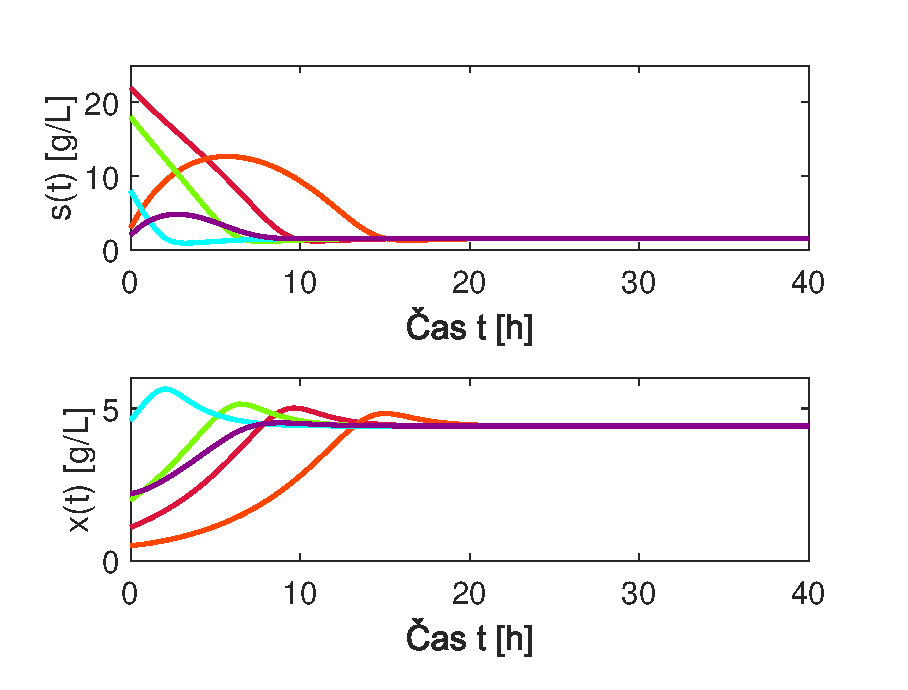
\includegraphics[width=\linewidth]{images/phase1_monod}
		\caption{Časový priebeh koncentrácie biomasy $ x(t) $ a substrátu $ s(t) $.}
		\label{fig:fazovy_vyber_monod}
	\end{subfigure}
	\begin{subfigure}[b]{0.49\textwidth}
		\centering
		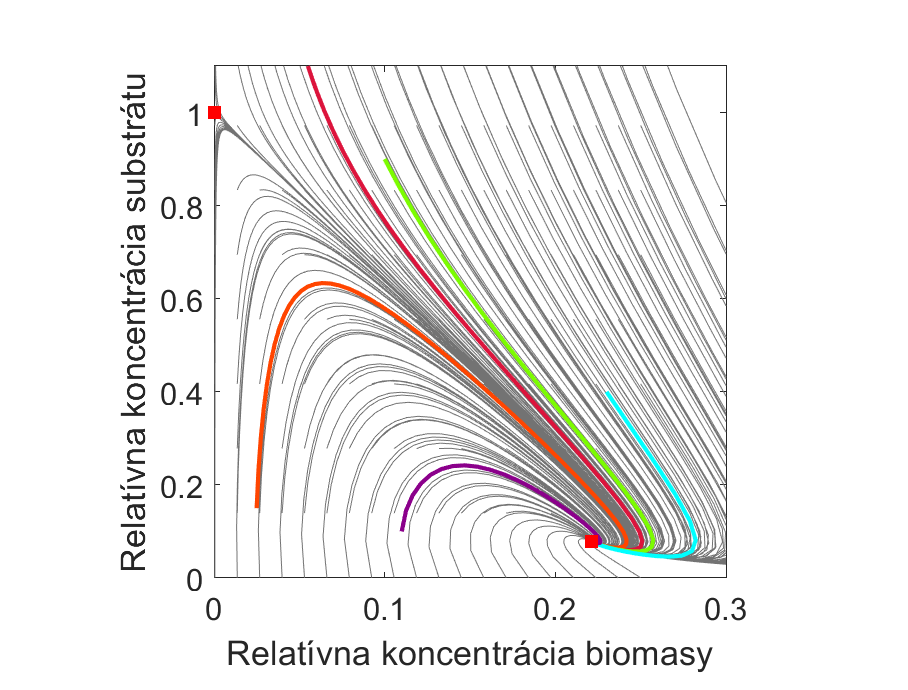
\includegraphics[width=\linewidth]{images/phase2_monod}
		\caption{Fázový diagram. Relatívny pomer vzhľadom na $ s_{in} $.}
		\label{fig:fazovy_monod}
	\end{subfigure}
	\caption{Stabilita a ustálený stav Monod modelu. Nastavenie parametrov modelu: $ \mu_{m} = 0.8\si{\per\hour}, \nu = 0.5\si{\per\hour}, K_{M} = 1.2\si{\gram\per\liter}, Y_{x} = 0.4, Y_{p} = 1, s_{in} = 20\si{\gram\per\liter} $.}
	\label{fig:stabilita_monod}
\end{figure}

Na  fázovom diagrame Monod modelu (Obr. \ref{fig:fazovy_monod}), môžeme vidieť oba ustálené stavy. Ak zvolíme začiatočné podmienky rôzne od nuly (najmä pri koncentrácii biomasy -- vedú k triviálnemu riešeniu a systémom bude pretekať čerstvý substrát) pri konštantnej rýchlosti riedenia menšej alebo rovnej ako špecifická rýchlosť rastu, sa vždy dostaneme do toho istého ustáleného stavu.
\begin{figure}
	\centering
	\begin{subfigure}[b]{0.49\textwidth}
		\centering
		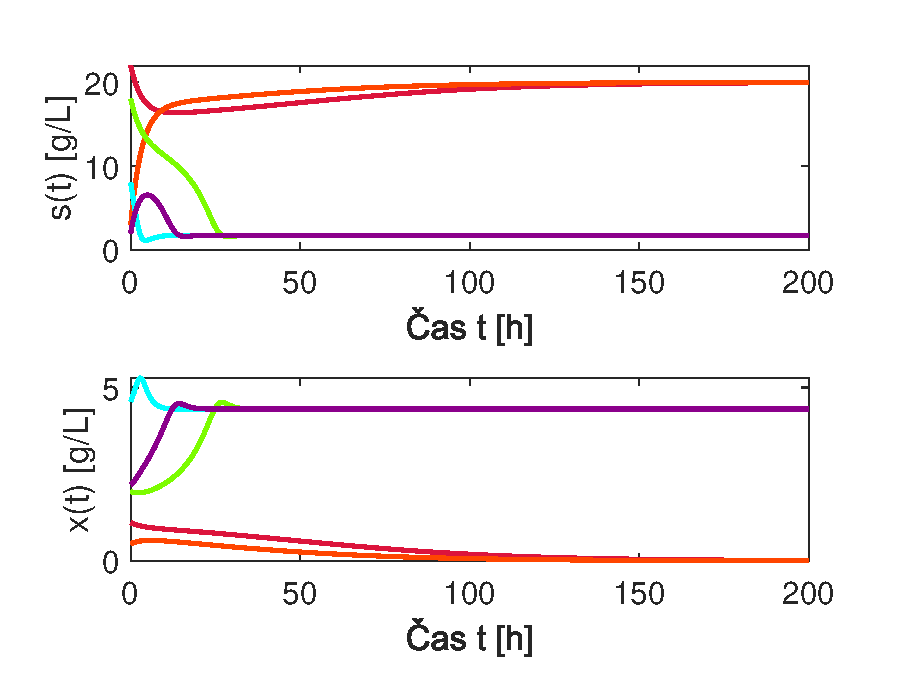
\includegraphics[width=\linewidth]{images/phase1_haldane}
		\caption{Časový priebeh koncentrácie biomasy $ x(t) $ a substrátu $ s(t) $.}
		\label{fig:fazovy_vyber_haldane}
	\end{subfigure}
	\begin{subfigure}[b]{0.49\textwidth}
		\centering
		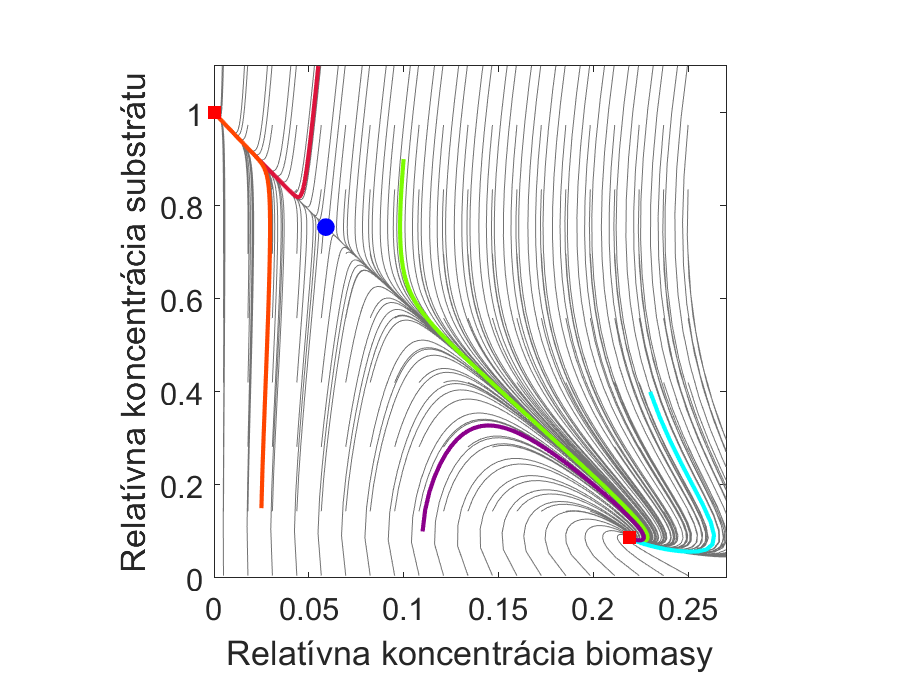
\includegraphics[width=\linewidth]{images/phase2_haldane}
		\caption{Fázový diagram. Relatívny pomer vzhľadom na $ s_{in} $.}
		\label{fig:fazovy_haldane}
	\end{subfigure}
	\caption{Stabilita a ustálený stav Haldane modelu. Nastavenie parametrov modelu: $ \mu_{m} = 0.8\si{\per\hour}, \nu = 0.5\si{\per\hour}, K_{M} = 1.2\si{\gram\per\liter}, K_{I} = 20\si{\gram\per\liter}, Y_{x} = 0.4, Y_{p} = 1, s_{in} = 20\si{\gram\per\liter}$.}
	\label{fig:stabilita_haldane}
\end{figure}

Model s inhibíciou vykazuje odlišné správanie. Na fázovom diagrame, Obr.\ref{fig:fazovy_haldane}, môžeme sledovať už dva nenulové stavy a jeden nulový. Výsledkom triviálneho riešenia je \aps{výplach}, ktorý vedie k nulovej koncentrácii biomasy. Ako si môžeme všimnúť, vždy keď je rýchlosť rastu biomasy pomalšia ako je odtok suspenzie zo systému, dostaneme sa do výplachu. To môžeme vidieť na trajektórii zobrazenej ružovou alebo oranžovou farbou na Obr. \ref{fig:fazovy_haldane}. Ostali dva netriviálne stavy, z ktorých jeden je nestabilný (modrý kruh) a druhý je stabilný (červený štvorec). V okolí nestabilného stavu môžu nastať dva prípady a to v závislosti od počiatočných podmienok. Ak sa na Obr. \ref{fig:spec_rychl_rastu} nachádzame v okolí nestabilného stavu od neho naľavo (napr. koncentrácia substrátu $ s = 12\si{\gram\per\liter} $), to znamená, že rýchlosť rastu biomasy je väčšia ako odtok suspenzie, dostaneme sa do nenulového ustáleného stavu. Ak sa nachádzame viac napravo (napr. koncentrácia substrátu $ s = 18\si{\gram\per\liter} $), dostaneme sa do výplachu. V skutočnosti by sme to mohli interpretovať aj nasledovne. Ak sa nachádzame v okolí nestabilného stavu naľavo ($ s = 12\si{\gram\per\liter} $), to znamená, že v dôsledku inhibície nám odumierajú niektoré slabšie mikroorganizmy, ale stále je v systéme dostatok takých, ktoré dokážu znížiť množstvo substrátu v prospech nárastu biomasy a produktu. Tým pádom nám klesne koncentrácia substrátu (pokles koncentrácie substrátu bude sprevádzaný aj poklesom koncentrácie biomasy) a dostaneme sa do stabilného ustáleného stavu. Ak sa však nachádzame napravo od nestabilného stavu ($ s = 18\si{\gram\per\liter} $), letalita v dôsledku vysokého osmotického tlaku je omnoho väčšia ako vitalita mikroorganizmov a postupne inklinujeme k stavu vymytia.

Táto odlišnosť v správaní Monod a Haldane modelu je veľmi problematická. V prvom rade si treba uvedomiť, že dynamika systému oboch modelov je do určitého bodu totožná, čo nám vôbec neuľahčuje výber vhodného modelu. V prípade, že si zvolíme nesprávny model, napr. Monod model a naše zariadenie bude vykazovať aj inhibičný efekt, teda Haldane model, tak pri optimalizácii alebo riadení pomocou takéhoto modelu sa môže veľmi ľahko stať, že uvedieme naše zariadenie do nenávratného stavu vymytia. V skutočnosti, vždy budeme zaznamenávať rozdiely v správaní zariadenia a modelu, pretože nedokážeme presne opísať správanie živých organizmov. Z tohto dôvodu sa treba vysporiadať s touto problematikou a vhodným adeptom sa javí byť hybridné modelovanie. 
	\section{Ekonomická optimalizácia}
V tejto časti zhrnieme hlavný cieľ tejto práce a to optimalizáciu prietokového biochemického reaktora pomocou hybridného modelovania s využitím metódy garantovaného odhadu parametrov. Ukážeme, na akom princípe bude takýto hybridný model fungovať a porovnáme ho s inými metódami, ktoré sa tak isto vedia vysporiadať s úlohou optimalizácie zariadenia. Najskôr, však potrebujeme zadefinovať problematiku.

Majme fiktívne zariadenie prietokového biochemického reaktora, ktoré vieme simulovať Monod modelom. Parametre tohto modelu, ako aj ich veľkosť, sú uvedené v Tabuľke \ref{tab:case_study_monod_params}. Našim cenným produktom bude samotná biomasa (napr. pekárenské droždie), takže sa budeme snažiť maximalizovať produkciu biomasy, ale na druhej strane budeme požadovať, aby sme pri tom minuli čo najmenej substrátu. Ak túto vetu transformujeme na matematický opis, mohli by sme získať takúto optimalizačnú úlohu
\begin{equation}
	\label{eq:chemostat_opt_general}
	\begin{split}
		\min_{D} &\quad D\left(1-\bar{x}\right), \\
		\text{s.t.} &\quad \bar{x} = f(D,\bar{s})
	\end{split}
\end{equation}
kde $ \bar{x} $ je ustálený stav koncentrácie biomasy a $ \bar{s} $ je ustálený stav koncentrácie substrátu. Funkcia $ f(D,\bar{s}) $ vyjadruje vzťah medzi hodnotou ustáleného stavu koncentrácie biomasy, substrátu a rýchlosti riedenia. Funkciu $ f(D,\bar{s}) $ získame z mechanického modelu, ktorým sme opísali správanie nášho zariadenia. Tento model predstavuje Haldane model resp. model s inhibíciou, ktorého parametre sú tak isto uvedené v Tabuľke \ref{tab:case_study_monod_params}. 

\begin{table}
	\centering
	\caption{Nastavenie parametrov Monod a Haldane modelu.}
	\label{tab:case_study_monod_params}
	\begin{tabular}{lll}
		\hline
		\textbf{Parameter} & \textbf{Symbol} & \textbf{Veľkosť} \\
		\hline
		Maximálna špecifická rýchlosť rastu & $\mu_{m}$ & 0.53\si{\per\hour} \\
		Michaelisova konštanta & $K_{M}$ & 1.20\si{\gram\per\liter} \\
		Rýchlosť tvorby produktu & $ \nu $ & 0.50\si{\per\hour} \\
		Výťažok (biomasa) & $Y_{x}$ & 0.40\\
		Výťažok (produkt) & $Y_{p}$ & 1.00\\
		Objem reaktora & $V$ & 3.33\si{\liter} \\
		Prietok substrátu/suspenzie & $F$ & 1.00\si{\liter\per\hour} \\
		Koncentrácia substrátu na vstupe & $s_{in}$ & 20.00\si{\gram\per\liter} \\
		Koeficient inhibície & $ K_{I} $ & 70.00\si{\gram\per\liter}\\
		\hline
	\end{tabular}
\end{table}

Ustálený stav Haldane modelu môžeme napísať v tvare
\begin{align}
	&0 = \left(\mu(\bar{s}) - D\right)\bar{x}, \label{eq:tmp_haldane_x_ss}\\
	&0 = D\left(s_{in} - \bar{s}\right) - \frac{1}{Y_{x}}\mu(\bar{s})\bar{x} - \frac{1}{Y_{p}}\nu \bar{x}, \label{eq:tmp_haldane_s_ss}\\
	&0 = \nu \bar{x} - D\bar{p} \label{eq:tmp_haldane_p_ss}.
\end{align}
Z rovnice \eqref{eq:tmp_haldane_x_ss} sme získali dve riešenia -- triviálne, ak koncentrácia biomasy bude v každom čase nulová; netriviálne, ak špecifická rýchlosť rastu bude rovná rýchlosti riedenia. Potom pre špecifickú rýchlosť rastu môžeme písať 
\begin{equation}
	\mu(\bar{s}) = D = \mu_{m}\frac{\bar{s}}{K_{M} + \bar{s} + \frac{\bar{s}^2}{K_{I}}} \quad \Longrightarrow \quad
	\frac{D}{K_{I}}\bar{s}^2 + (D-\mu_{m})\bar{s} + DK_{M} = 0.
\end{equation}
Riešením tejto kvadratickej rovnice dostaneme dve riešenia, pričom fyzikálny zmysel má iba jedno
\begin{equation}
	\label{eq:haldane_subs_ss}
	\bar{s} = -K_{I}\frac{\left(D-\mu_{m}\right) + \sqrt{\left(D-\mu_{m}\right)^2 - 4\frac{D^2}{K_{I}}K_{M}}}{2D}. 
\end{equation}
Takto sme získali rovnicu ustáleného stavu koncentrácie substrátu. Ustálený stav koncentrácie biomasy vieme odvodiť z rovnice \eqref{eq:tmp_haldane_s_ss}
\begin{equation}
\label{eq:haldane_biomass_ss}
	0 = D\left(s_{in}-\bar{s}\right) - \left(\frac{1}{Y_{x}}D + \frac{1}{Y_{p}}\nu\right)\bar{x} \quad \Longrightarrow \quad
	\bar{x} = \frac{D\left(s_{in}-\bar{s}\right)}{\frac{1}{Y_{x}}D + \frac{1}{Y_{x}}\nu}. 
\end{equation}
A nakoniec posledná rovnica \eqref{eq:tmp_haldane_p_ss} definuje hodnotu ustáleného stavu produktu
\begin{equation}
\label{eq:haldane_product_ss}
	0 = \nu \bar{x} - D\bar{p} \quad \Longrightarrow \quad \bar{p} = \frac{\nu}{D}\bar{x}.
\end{equation}
Keďže už vieme aký predpis má funkcia $ f(D,\bar{s}) $, môžeme optimalizačnú úlohu \eqref{eq:chemostat_opt_general} upraviť do nasledujúceho tvaru 
\begin{equation}
\label{eq:chemostat_opt_w_ss}
	 \begin{split}
		 \min_{D} &\quad D\left(1-\alpha\bar{x}\right), \\
		 \text{s.t.} &\quad \bar{x} = \frac{D\left(s_{in}-\bar{s}\right)}{\frac{1}{Y_{x}}D + \frac{1}{Y_{x}}\nu} \\
		 &\quad \bar{s} = -K_{I}\frac{\left(D-\mu_{m}\right) + \sqrt{\left(D-\mu_{m}\right)^2 - 4\frac{D^2}{K_{I}}K_{M}}}{2D}
	 \end{split}
\end{equation}
Kvôli problémom s definičným oborom účelovej funkcie Haldane modelu (viď rovnicu \eqref{eq:haldane_subs_ss}), sme museli pridať do účelovej funkcie koeficient $ \alpha $, ktorého veľkosť sme empiricky zvolili rovný $ \alpha = 0.5 $. Toto nám umožnilo rozšíriť definičný obor aspoň po oblasť optimálnej hodnoty Monod modelu.

Treba zdôrazniť, že správanie takto nastaveného Haldane modelu je naprosto odlišné od nášho zariadenia, pretože za určitých podmienok sa prejavuje inhibícia v dôsledku vysokej koncentrácie substrátu, a preto bude mať optimum účelovej funkcie niekde inde ako naše zariadenie simulované Monod modelom, ako to vidno na Obr. \ref{fig:cost_fun_comparison}. To znamená, že ak by sme sa riadili iba týmto nepresným mechanickým modelom, naše zariadenie by vôbec nepracovalo najefektívnejšie ako to je len možné. Z tohto dôvodu sa budeme snažiť navrhnúť hybridný model tak, aby dokázal vyrovnať rozdiel medzi nominálnym modelom a zariadením. Vhodnou štruktúrou hybridného modelu na riešenie tejto problematiky je paralelné zapojenie.

\begin{figure}
	\centering
	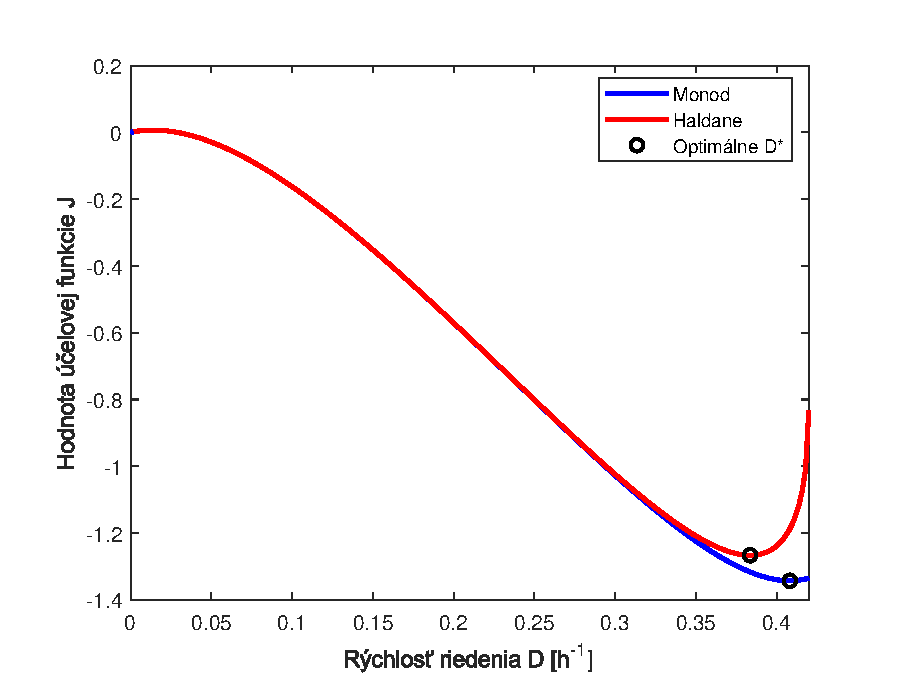
\includegraphics[width=0.7\linewidth]{images/cost_fun_comparison}
	\caption{Porovnanie účelovej funkcie Monod a Haldane modelu. Zariadenie je simulované Monod modelom a Haldane model predstavuje náš nepresný mechanický model.}
	\label{fig:cost_fun_comparison}
\end{figure}

\textbf{Použitie hybridných modelov.} Na začiatku treba spomenúť, že ide o iteračnú metódu, i keď hybridné modely majú tú výhodu, že dátovú časť by sme vedeli natrénovať na údajoch zo zariadenia aj bez iteračného prístupu, ale nemali by sme zaručenú úspešnosť výsledku. 

Princíp optimalizácie demonštrujeme na situácii, keď dokážeme merať iba koncentráciu substrátu. Z ustáleného stavu, spravíme skokovú zmenu v rýchlosti zrieďovania $ D $, v prípade zariadenia aj modelu. Na základe rozdielu $ \Delta_{s} $ týchto dát
\begin{equation}
	\Delta_{s} = \tilde{s} - s,
\end{equation}
kde $ \tilde{s} $ sú údaje získané zo zariadenia a $ s $ predstavuje údaje z nominálneho modelu, identifikujeme dátový model pomocou metódy GOP. V prípade, že by našim dátovým modelom bol FIR, môžeme využiť rovnice \eqref{eq:gpe_fir_min_rad} a \eqref{eq:gpe_fir_param_est}. ARX model by sme mohli identifikovať pomocou \eqref{eq:gpe_arx_min_rad} a \eqref{eq:gpe_arx_param_est}. Takto natrénovaný dátový model využijeme na korekciu ustáleného stavu substrátu nominálneho modelu v optimalizačnej úlohe \eqref{eq:chemostat_opt_w_ss}. Po úprave by sme ju mohli formulovať nasledovne
\begin{equation}
\label{eq:hybrid_opt_subs}
	\begin{split}
		\min_{D} &\quad D\left(1-\alpha\bar{x}\right), \\
		\text{s.t.} &\quad \bar{x} = \frac{D\left(s_{in}-s_{corr}\right)}{\frac{1}{Y_{x}}D + \frac{1}{Y_{x}}\nu} \\
		&\quad s_{corr} = \bar{\Delta}_{s}(D) + \bar{s}\\
		&\quad \bar{s} = -K_{I}\frac{\left(D-\mu_{m}\right) + \sqrt{\left(D-\mu_{m}\right)^2 - 4\frac{D^2}{K_{I}}K_{M}}}{2D}
	\end{split}
\end{equation}
kde $ \bar{\Delta}_{s}(D) $ je ustálený stav dátového modelu. Riešenie tejto upravenej optimalizačnej úlohy nám vráti novú hodnotu optimálneho $ D $, odlišnú od predchádzajúcej a túto využijeme na generovanie novej skokovej zmeny, nových dát. 

Takto postupujeme, až dokým neskonvergujeme k optimálnej hodnote rýchlosti riedenia $ D^{\star} $ zariadenia. V tomto bode by ustálený stav dátového modelu $ \bar{\Delta}_s $ mal nadobudnúť hodnotu
\begin{equation}
	\bar{\Delta}_s = \hat{s}\left(D^{\star}\right) - \bar{s}\left(D^{\star}\right),
\end{equation} 
kde $ \hat{s}\left(D^{\star}\right) $ je hodnota ustáleného stavu koncentrácie substrátu zariadenia a $ \bar{s}\left(D^{\star}\right) $ nominálneho modelu pri rýchlosti riedenia $ D^{\star} $.

Ak by nastala situácia, že zo zariadenia vieme získať iba údaje o koncentrácii biomasy, princíp fungovania hybridného modelu by sa nezmenil. Zmenili by sa iba dáta resp. dátové modely. Zaznamenali by sme rozdiel v koncentrácii biomasy $ \Delta_{x} $ a pripravili trénovacie dáta ako
\begin{equation}
	\Delta_{x} = \tilde{x} - x,
\end{equation} 
kde $ \tilde{x} $ sú namerané údaje zo zariadenia a $ x $ sú dáta z nominálneho modelu. Na základe týchto údajov by sme identifikovali dátový model, ktorý by sme použili na úpravu ustáleného stavu biomasy $ \bar{x} $ nominálneho modelu v optimalizačnej úlohe nasledovným spôsobom
\begin{equation}
\label{eq:hybrid_opt_bio}
	\begin{split}
		\min_{D} &\quad D\left(1-\alpha\left(\bar{x}+\bar{\Delta}_{x}(D)\right)\right), \\
		\text{s.t.} &\quad \bar{x} = \frac{D\left(s_{in}-\bar{s}\right)}{\frac{1}{Y_{x}}D + \frac{1}{Y_{x}}\nu} \\
		&\quad \bar{s} = -K_{I}\frac{\left(D-\mu_{m}\right) + \sqrt{\left(D-\mu_{m}\right)^2 - 4\frac{D^2}{K_{I}}K_{M}}}{2D}
	\end{split}
\end{equation}
kde $ \bar{\Delta}_{x}(D) $ predstavuje ustálený stav dátového modelu.

Avšak, medzi dátami o koncentrácii substrátu a biomasy je kvalitatívny rozdiel, a tým je vplyv šumu merania. Zatiaľ čo, meranie koncentrácie substrátu nebýva zaťažené veľkou chybou merania, koncentrácia biomasy má výrazne vyššiu fluktuáciu. Preto sa najčastejšie z výstupných prúdov meria koncentrácia substrátu. 

Aby sme vedeli zhodnotiť kvalitu prístupu k optimalizácii nášho zariadenia použitím hybridných modelov, porovnáme tento prístup s ďalšími dvoma metódami. Sú nimi dvojkroková optimalizácia a schéma úpravy modifikátora. Oba tieto prístupy patria k iteračným metódam.

\textbf{Dvojkroková optimalizácia.}
V prvej fáze sa zameriame na odhad parametrov nominálneho modelu. Treba si uvedomiť, že nepotrebujeme odhadovať všetky parametre modelu, pretože niektoré z nich vieme získať meraním ako jednotlivé výťažky $ Y_{x}, Y_{p} $, rýchlosť tvorby produktu $ \nu $, koncentráciu substrátu na vstupe $ s_{in} $. Tieto parametre si vopred zadefinujeme a budú mať takú veľkosť, ako udáva Tabuľka \ref{tab:case_study_monod_params}. Zvyšné parametre modelu, maximálnu špecifickú rýchlosť rastu $ \mu_{m} $, Michaelisovu konštantu $ K_{M} $ a koeficient inhibície $ K_{I} $, tzv. kinetické členy, budeme odhadovať. Na základe nameraných údajov zo skokovej zmeny môžeme zvoliť dve cesty.

V prípade, že disponujeme dátami koncentrácie biomasy aj substrátu, môžeme optimalizačný problém odhadu parametrov sformulovať nasledovne
\begin{equation}
\label{eq:twostep_der_app}
	\begin{split}
		\min_{\mu_{m},K_{M}} \quad &\sum_{i=1}^{N} \left(\Delta_{i} - \left(\mu(\tilde{s}_{i}) - D\right)\tilde{x}_{i}\right)^2, \\
		\text{s.t.} \quad &\Delta_{i} = \frac{\tilde{x}_{i} - \tilde{x}_{i-1}}{t_{i} - t_{i-1}} \\
		\quad &\mu(\tilde{s}_{i})=\mu_{m}\frac{\tilde{s}_{i}}{K_{M} + \tilde{s}_{i} + \frac{\tilde{s}_{i}^2}{K_{I}}}
	\end{split}
\end{equation} 
pre všetky $ i \in \lbrace 1,2,3,\dots,N \rbrace $, kde $ \tilde{x}_{i} $ predstavuje nameranú hodnotu koncentrácie biomasy v $ i $--tom kroku v čase $ t_i $, $ \tilde{s}_{i} $ substrátu a $ \Delta_{i} $ predstavuje spätnú diferenciu v $ i $--tom kroku. Táto metóda aproximuje údaje o derivácii časového priebehu koncentrácie biomasy. Najväčšou prekážkou pre takýto prístup je samotný šum merania a čím väčší bude jeho rozptyl, tým ďalej budeme od skutočnej derivácie.

Druhý prístup odhaduje parametre samotných diferenciálnych rovníc nominálneho modelu na základe nameraných údajov koncentrácie substrátu $ \tilde{s} $. Zatiaľ čo formulácia optimalizačného problému sa príliš nezmení, zložitosť výpočtu sa výrazne zvýši. V tomto prípade je nutné, v každom nameranom bode, niekoľkokrát numericky vyhodnotiť priebehy koncentrácie biomasy aj substrátu a porovnať ich s nameraným signálom  tak, aby sme získali optimálne riešenie. Túto problematiku by sme mohli sformulovať následovne
\begin{equation}
\label{eq:twostep_diff_pe}
	\begin{split}
		\min_{\mu_{m},K_{M}} \quad & \sum_{i=1}^{N} \left(\tilde{s}_{i}-s_{i}\right)^2, \\
		\textrm{s.t.} \quad & \dot{s} = D(s_{in}-s)-\frac{1}{Y_x}\mu(s)x-\frac{1}{Y_p}\nu x \\
		& \dot{x} = (\mu(s)-D)x \\
		& \mu(s)=\mu_{m}\frac{s}{K_{M} + s + \frac{s^2}{K_{I}}} \\
		& s(0) = s_0 \\
		& x(0) = x_0
	\end{split}
\end{equation}
pre všetky $ i \in \lbrace 1,2,3,\dots,N \rbrace $, kde $ s_{i} $ je koncentrácia substrátu v $ i $--tom kroku vypočítaná na základe nominálneho modelu.

V druhej fáze na základe identifikovaného nominálneho modelu určíme optimálnu rýchlosť riedenia resp. prietok v danom kroku podľa rovnice \eqref{eq:chemostat_opt_w_ss}. Prvú a druhú fázu budeme cyklicky opakovať na pribúdajúcich dátach, až kým neskonvergujeme k skutočnému optimálnemu prietoku zariadenia.

\textbf{Schéma úpravy modifikátora.}
Táto metóda upravuje gradient účelovej funkcie \eqref{eq:chemostat_opt_w_ss}, už identifikovaného nominálneho modelu, na základe nameraných údajov koncentrácie biomasy zo zariadenia. Postupovať budeme nasledovne.

Začneme tým, že si označíme našu účelovú funkciu v $ k $--tom kroku resp. iterácii ako
\begin{equation}
\label{eq:chemostat_cost_fun}
	J_{k} = D_{k}\left(1-\alpha\bar{x}_{k}\right).
\end{equation}
Keďže nepoznáme matematický opis skutočného zariadenia a potrebujeme získať informáciu o gradiente jeho účelovej funkcie $ \nabla_{P}J_{k} $, musíme ho odhadnúť pomocou spätnej diferencie
\begin{equation}
	\nabla_{P}J_{k} = \frac{J_{k} - J_{k-1}}{D_{k} - D_{k-1}} = \frac{\left(D-D\alpha\hat{x}\right)_{k} - \left(D-D\alpha\hat{x}\right)_{k-1}}{D_{k} - D_{k-1}}
\end{equation}
kde $ \hat{x} $ sú namerané údaje ustáleného stavu koncentrácie biomasy v $ k $--tom resp. $ k-1 $ kroku pri príslušnej zrieďovacej rýchlosti $ D_{k} $ a $ D_{k-1} $. Úprava modifikátora, ako to definuje rovnica \eqref{eq:mas_correction}, je daná rozdielom gradientov účelových funkcií zariadenia $ \nabla_{P}J_{k} $ a nominálneho modelu $ \nabla_{N}J_{k} $ 
\begin{equation}
\label{eq:mas_chemostat_modifierValue}
	\Delta_k = \nabla_{P}J_{k} - \nabla_{N}J_{k}.
\end{equation}
Gradient účelovej funkcie nominálneho modelu získame deriváciou rovnice \eqref{eq:chemostat_cost_fun} podľa rýchlosti riedenia $ D $
\begin{align}
	&\nabla_{N}J = 1 - \alpha\left(\bar{x}+D\pder{\bar{x}}{D}\right), \text{kde}\\
	&\pder{\bar{x}}{D} = \frac{\left(\frac{D}{Y_{x}} + \frac{\nu}{Y_{p}}\right)\left(\bar{s}-s_{in}+D\pder{\bar{s}}{D}\right) - \frac{D\left(\bar{s}-s_{in}\right)}{Y_{x}}}{\left(\frac{D}{Y_{x}} + \frac{\nu}{Y_{p}}\right)^2},	\\
	&\pder{\bar{s}}{D} = f(D,K_{M},K_{I},\mu_{m}),
\end{align}
kde $ \pder{\bar{s}}{D} $ sme nechali vo všeobecnom tvare kvôli zložitosti výrazu a ustálené hodnoty koncentrácie biomasy $ \bar{x} $ a substrátu $ \bar{s} $ sú definované vzťahmi \eqref{eq:haldane_biomass_ss} a \eqref{eq:haldane_subs_ss}. Je zrejmé, že gradient tejto funkcie $ \nabla_{N}J_{k} $ musíme vypočítať na základe rovnakých údajov $ D_k $ v kroku $ k $. 

Problematickým faktorom pri odhade gradientu účelovej funkcie zariadenia je šum merania, ktorý bude vždy prítomný. Preto aktuálnu hodnotu modifikátora v $ k $--tom kroku $ \lambda_k $ nastavíme vhodným váhovaním minulých hodnôt modifikátora $ \lambda_{k-1} $ a aktuálnej hodnoty rozdielu $ \Delta_{k} $ tak ako udáva rovnica \eqref{eq:mas_weight}
\begin{equation*}
	\lambda_k = c\lambda_{k-1} + \left(1 - c\right)\Delta_{k},
\end{equation*}
kde $ c $ je váhový koeficient. Takto vypočítaná hodnota modifikátora $ \lambda_k $ sa pripočíta ku gradientu účelovej funkcie nominálneho modelu $ \nabla_{N}J $, kde po integrácii dostaneme
\begin{equation}
	J_{k} = D\left(1-\alpha\bar{x}\right) + D\lambda_k.
\end{equation}
Optimalizačnú úlohu potom zostavíme na základe tejto upravenej rovnice
\begin{equation}
	\begin{split}
		\min_{D} &\quad D\left(1-\alpha\bar{x}\right) + D\lambda_k, \\
		\text{s.t.} &\quad \bar{x} = \frac{D\left(s_{in}-\bar{s}\right)}{\frac{1}{Y_{x}}D + \frac{1}{Y_{x}}\nu} \\
		&\quad \bar{s} = -K_{I}\frac{\left(D-\mu_{m}\right) + \sqrt{\left(D-\mu_{m}\right)^2 - 4\frac{D^2}{K_{I}}K_{M}}}{2D}
	\end{split}
\end{equation}
ktorou získame optimálnu rýchlosť riedenia $ D $ resp. prietok $ F $ v príslušnej iterácii. Na základe ďalších hodnôt o ustálených stavoch aktualizujeme hodnotu modifikátora $ \lambda_k $, ktorá v najideálnejšom prípade konverguje k hodnote
\begin{equation}
	\label{eq:mas_opt_lambda}
	\lambda_k = \nabla_{P}J\left(D^{\star}\right) - \nabla_{N}J\left(D^{\star}\right).
\end{equation} 
Ak modifikátor nadobudne túto hodnotu, dosiahli sme optimálny chod zariadenia pri $ D^{\star} $. Treba pripomenúť, že rýchlosť konvergencie, ako aj jej kvalita, záležia od voľby váhového koeficientu $ c $. Pomalá konvergencia nemusí byť vhodná pre procesy, kde dosiahnutie ustáleného stavu trvá hodiny až dni, ale je presná. Na druhej strane rýchla konvergencia kmitá okolo optimálnej hodnoty a často s veľkou amplitúdou.

	
% conclusions
\chapter{Výsledky}
thesis conclusions

% Appendices (Prílohy) comment by "%" if not neccesary
\appendix
\chapter{Resumé}
V oblasti automatizácie sa často stretávame s problematikou nezhody matematického opisu so skutočným zariadením. Tieto nezhody sú väčšinou spôsobené rôznymi aproximáciami, ktorými sa snažíme v jednoduchosti, matematicky opísať správanie komplexného systému. Podobne je to aj v prípade biochemických reaktorov. Vlastnosti biochemických reaktorov sú výlučne stanovené správaním živých organizmov, ktoré ponúkajú široké spektrum dynamického správania. Ich správanie sa líši nielen v závislosti od typu mikroorganizmu, ale aj v rámci jedného druhu, čo vedie k problémom s modelovaním takýchto procesov a v konečnom dôsledku môžeme skončiť s matematickým opisom, ktorý je rôzny od skutočnosti. 

Odlišnosť v správaní skutočného biochemického reaktora a jeho modelu predstavuje závažný problém, hlavne v situácii, keď sa snažíme zabezpečiť efektívnu prevádzku zariadenia. Veľa vedeckých publikácii sa venuje práve tejto tématike, ale riešenia, ktoré ponúkajú, ako napr. dvojkroková optimalizácia alebo úprava účelovej funkcie použitím modifikátora, sú často veľmi komplikované na realizáciu alebo vedú k nepresným výsledkom. Z tohto dôvodu sme sa rozhodli, že navrhneme odlišný prístup k problematike optimalizácie prietokového biochemického reaktora, pomocou nepresného mechanického modelu, ktorý je založený na hybridnom modelovaní s využitím garantovaného odhadu parametrov.

Väčšina metód nerieši problematiku voľby rádu modelu, ktorá je esenciálnou úlohou pri identifikácii dátových modelov a výrazne komplikovanejšou ako odhad parametrov modelu. Garantovaný odhad parametrov nám ponúka informácie o minimálnom ráde (štruktúre) modelu a v spojení s Pareto frontom sme dokázali posúdiť aj kvalitu modelov vyšších rádov. Vhodný rád modelu sme potom zvolili na základe kompromisu medzi presnosťou odhadu modelu a jeho maximálnym rozptylom odhadu. V ďalšej časti identifikácie pomocou GOP sme získali garantovanú oblasť všetkých možných riešení, v rámci stanovenej chyby modelu. Táto oblasť, ktorá je určená minimálnou a maximálnou realizáciou modelu nám zaručuje, že skutočné riešenie leží v vo vnútri.  

Ukázali sme, že takto dokážeme nájsť vhodné dátové modely, či už FIR alebo ARX, na opis údajov, ktoré vyjadrujú rozdiel koncentrácie biomasy alebo substrátu medzi skutočným zariadením (Monod model) a nominálnym modelom (Haldane model). Dynamika týchto modelov bola odlišná, ale v predikcií ustálených stavov boli FIR aj ARX model rovnako dobré. Preto sme sa rozhodli, že pri konštrukcii hybridných modelov sa zameriame iba na FIR modely.

Výsledky experimentov hybridného modelovania nás priviedli k záveru, že hybridné modelovanie môže byť použité na optimalizáciu prevádzky biochemického reaktora. Z dát, ktoré dokážeme získať zo zariadenia, sme odvodili dva hybridné modely, jeden substrátový a druhý biomasový. Oba viedli k rovnakým výsledkom, ak sme upravili vplyv chyby merania koncentrácie biomasy tak, aby bola porovnateľná s chybou merania koncentrácie substrátu, vzhľadom na generované skokové zmeny. Uviedli sme niekoľko prístupov v rámci hybridného modelovania, ktoré sa dajú aplikovať na spomínanú problematiku. Iteračná metóda dokázala skonvergovať v priebehu pár krokov, ale dostala sa iba do okolia optima. Ak sme dátovú časť hybridného modelu natrénovali na dopredu známych dátach, tak sme sa dostali do presného optimálneho stavu zariadenia. Ale ak by sme pridali dáta zo skokových zmien pri väčších hodnotách rýchlosti riedenia, tak s veľkou pravdepodobnosťou by sme optimálny stav presiahli. Nevýhodou tohto prístupu je aj skutočnosť, že ak zapojíme vopred natrénovaný model do iteračnej optimalizácie, tak po niekoľkých iteráciách sa ustálený stav zariadenia vzdiali od optimálneho. Je to spôsobené tým, že po určitom čase už iteračný prístup nedokáže vygenerovať informačne výdatné dáta na identifikáciu dátového modelu. Najdôležitejším výsledkom v rámci hybridného modelovania je, že aj keby hybridný model predikoval presný rozdiel v koncentrácii zariadenia a nominálneho modelu v optimálnom režime, nikdy by sme nedosiahli skutočné optimum zariadenia, ale dostali by sme sa do veľmi blízkeho okolia.

Dvojkroková optimalizácia dokázala v niektorých špeciálnych prípadoch (najmä na začiatku optimalizačného procesu, keď sme mali k dispozícii málo dát) skonvergovať k optimu zariadenia, iba pomocou odhadu kinetických členov nominálneho modelu, pretože zväčšovaním hodnoty inhibičného koeficientu, vieme zmenšiť rozdiely v správaní Monod a Haldane modelu.
V ďalších iteráciách, kedy narastal počet dát, teda sa zvyšovala presnosť odhadu, sa riešenia od optima vzdialili. Problematická situácia nastala najmä vtedy, ak koeficient inhibície $ K_I $ nadobudol hodnoty rádovo $ 10^{10}\si{\gram\per\liter} $. To viedlo k takému priebehu účelovej funkcie nominálneho modelu resp. iba jej časti, ktorá spôsobila problémy pri samotnom riešení optimalizačnej úlohy a výsledkom boli rýchlosti riedenia, ktoré dostali prietokový biochemický reaktor do stavu vymytia.

V teoretickej rovine, je schéma úpravy modifikátora jedinou z použitých metód, ktorá dokáže uviesť zariadenie do jeho optimálneho režimu v niekoľkých krokoch, aj napriek nepresnému matematickému opisu zariadenia. Rýchlosť konvergencie závisí od veľkosti váhového koeficientu $ c $, kde menšie hodnoty znamenajú rýchlejší priebeh konvergencie a naopak väčšie hodnoty pomalší. Situácia sa zmenila, ak sme začali uvažovať vplyv šumu merania. Ako sme ukázali, tak chyba merania mohla v niektorých situáciách pomôcť rýchlejšej konvergencii, ale ak bol šum merania výraznejší ako skoková zmena, vznikali oscilácie a nedokázali sme zabezpečiť konvergenciu k optimu, hlavne v iteráciách, kedy skutočný gradient účelovej funkcie bol rovný nule. Spoľahlivosť tejto metódy záleží na nastavení jej parametrov, čo vôbec nie je jednoduchá úloha, najmä v prípade biochemického reaktora, kde fluktuácia koncentrácie biomasy je veľmi výrazná.

Pri porovnaní jednotlivých metód pre niekoľko rôznych realizácií šumu merania sme zistili, že vo väčšine prípadov si problematikou optimalizácie prevádzky prietokového biochemického reaktora na základe nepresného mechanického modelu najlepšie poradila metóda s použitím hybridného modelovania, i keď od začiatku sme vedeli, že nás dostane iba do blízkeho okolia optima. V dvadsiatej iterácii sa hybridný model aj schéma úpravy modifikátora dostali do približne rovnakého ustáleného stavu. Rozdiel bol v tom, že zatiaľ čo metóde schéme úpravy modifikátora to trvalo celých 20 iterácii, čo v prípade biochemického reaktora predstavuje 1000 hodín, hybridné modely to zvládli za 5 iterácií, teda 250 hodín. Dvojkroková optimalizácia už v druhej iterácii uviedla zariadenie do optimálneho ustáleného stavu, ale v ďalších krokoch divergovala od optima do stavu vymytia.

Iteračný proces optimalizácie pomocou hybridných modelov by sa dal ešte vylepšiť. My sme ukázali, že korekcia ustálených stavov nominálneho modelu, nie je v spojní s iteračným prístupom najvhodnejším adeptom na optimalizáciu prevádzky. Ak by sme pristupovali k optimalizácii, v rámci hybridného modelovania, podobne ako schéma úpravy modifikátora, t.j. zmenou gradientu účelovej funkcie, je tu možnosť, že by sme takto dokázali dosiahnuť presné optimum. Podobne by sme mohli použiť hybridné modely na odhad ustálených stavov zariadenia, pomocou ktorých by schéma úpravy modifikátora vedela omnoho presnejšie odhadnúť gradient účelovej funkcie. Tieto hypotézy by však bolo potrebné overiť ďalším výskumom.

Hybridné modelovanie má niekoľko výhod oproti schéme úpravy modifikátora. Tým, že hybridné modely dokážu predikovať údaje zariadenia, vedeli by sme ich použiť pri riadení procesov, pričom riadenie by bolo omnoho kvalitnejšie ako s použitím samotného nominálneho modelu, čo sme aj demonštrovali na výsledkoch predikčných vlastností modelov. Šum merania nezohráva až takú významnú úlohu pri optimalizácii zariadenia. Dôležitú rolu pri tejto vlastnosti zohráva identifikácia dátových častí hybridných modelov pomocou metódy garantovaného odhadu parametrov. 

Kvalita hybridných modelov je stanovená kvalitou ich dátových častí. Ako sme ukázali, tak lineárne dátové modely ako FIR alebo ARX sa nedokážu efektívne vysporiadať s nelinearitou systému. Z tohto dôvodu vedú aj hybridné modely k nepresnej predikcii. S týmto problémom by sme sa pravdepodobne vedeli vysporiadať zmenou štruktúry hybridného modelu za sériovo--paralelnú, ale toto tvrdenie by bolo nutné overiť, čo môže byť námetom na ďalšiu prácu.

%----------------------------------------------------------------%
%  The Backmatter !! Do NOT change the structure!!               %
%----------------------------------------------------------------%
% Bibliography to TOC
% do not remove
\backmatter
\providebibliography
\bibliography{bibfile}

%----------------------------------------------------------------%
%   The end of the document                                      %
%----------------------------------------------------------------%
\end{document}
